\documentclass[a4paper,12pt]{report}
\usepackage[utf8]{inputenc}    %inputenc gère les accents
\usepackage[english]{babel}
\usepackage{appendix}
\usepackage{color}
\usepackage{graphicx} 
\usepackage{geometry}
\usepackage{pdfpages}
\usepackage{titlesec,lipsum}
\usepackage{hyperref}
\usepackage{indentfirst}
\usepackage{lmodern}
\usepackage[T1]{fontenc}
\usepackage{textcomp}
\usepackage{tcolorbox,listings}
\usepackage{fullpage}
\usepackage{color}
\usepackage{listings}

\addto\captionsfrench{\renewcommand{\chaptername}{Partie}}

\definecolor{grey}{rgb}{0.95, 0.95, 0.95}
\definecolor{green}{rgb}{0.271,0.545,0.455}

\lstset{
    backgroundcolor=\color{grey},
    breakatwhitespace=false,
    breaklines=true,
    captionpos=b,
    commentstyle=\color{green},
    deletekeywords={...},
    escapeinside={\%*}{*)},
    extendedchars=true,
    keepspaces=true,
    keywordstyle=\color{blue},
    language=Python,
    morekeywords={*,...},
    showspaces=false,
    showstringspaces=false,
    showtabs=false,
    stepnumber=1,
    stringstyle=\color{red},
    tabsize=4,
    title=\lstname,
}
 
\lstdefinestyle{frameStyle}{
    basicstyle=\footnotesize,
    numbers=left,
    numbersep=20pt,
    numberstyle=\tiny\color{black}
}
 
\tcbuselibrary{listings,skins,breakable}
 
\newtcblisting{customFrame}{
    arc=0mm,
    top=0mm,
    bottom=0mm,
    left=3mm,
    right=0mm,
    width=\textwidth,
    listing only,
    listing options={style=frameStyle},
    breakable
}

\geometry{left=2cm,right=2cm,top=3cm,bottom=4cm}
\makeatletter

\makeatother

\begin{document}

%%%%%%%%% PAGE DE GARDE %%%%%%%%%
\begin{center}
	\begin{center} 
\includegraphics[scale=1.2]{magendie.png} \textcolor{white}{ouiouioui}
	
\includegraphics[scale=0.5]{logo-universite-bordeaux.png}\end{center} \vfill
	\rule{0.75\textwidth}{2 pt} \vspace{0.9\baselineskip} \\ 
	\huge \textbf{Programming project report} \vspace{0.5\baselineskip}\\
	Analysis of electrophysiological and imaging data in the context of sensory information processing in autism \normalsize  \vspace{0.9\baselineskip} \\
	\rule{0.75\textwidth}{2pt} \\\vfill
	\large Alexandre \textsc{Cornier}, Martin \textsc{Drance}, Ali \textsc{Cuhadar}, Abdelghani \textsc{Neuhaus} \vspace{1.2\baselineskip}\\
	\textbf{Team leader} : Andreas \textsc{Frick}\\		
	\textbf{Project supervisor} : Marie \textsc{Beurton-Aimar} \vspace{1.2\baselineskip}\\
    \large{Master in Bioinformatics of Bordeaux}\\
    Year 2019- 2020 \\
    
	\thispagestyle{empty}
\end{center}


%%%%%%%%%% PAGE VIERGE %%%%%%%%%%%
\newpage
\topskip=0pt
\vspace*{\fill}

\begin{center}
    \noindent\textbf{A B S T R A C T}\\
    \rule{\linewidth}{0.1mm}
\end{center}
The neocortex plays a central role in processes such as the processing of sensory information, perception or even the control of motor activity. Cortical deficits therefore have dramatic neurological and psychiatric repercussions. The functioning of a cortical circuit results from the combination of the intrinsic properties of the neurons that compose it, the connectivity of these neurons and the properties of these connections. Integrating these three levels of functional complexity, one of the major challenges of contemporary neuroscience, is necessary for understanding the normal and pathological functioning of neural networks and the study of diseases of the central nervous system. \\
\newline Autism spectrum disorder (ASD) is estimated to affect one in fifty children. Atypical processing of sensory information (for example, tactile, visual and hearing information) is now considered a key phenotype of ASD and can be a key determinant of other basic autistic phenotypes. Information from the different senses are processed in the neocortical circuits and can be measured by electrophysiological or imaging approaches. Measurements of sensory information and perception processing could also provide objective biomarkers essential to complete the evaluation of social, communicational and cognitive/behavioral alterations and to quantify the therapeutic results. Today, re-education is possible depending on the level of severity but there is no targeted therapeutic approach. The object of the project is to improve the functioning of a tool intended to improve the treatment of autism therapeutically. \\
\newline The objective of this project is to develop software for an in-depth analysis of complex electrophysiological and imaging data. To achieve this, it will be couple existing software with the code produced in the project to extract the various characteristics of this data. \\[2mm]
\rule{\linewidth}{0.1mm}
	\thispagestyle{empty}

\vspace*{\fill}
\newpage

%%%%%%%%% SOMMAIRE %%%%%%%%%%
\setcounter{tocdepth}{1}
\setcounter{secnumdepth}{3}
\renewcommand{\contentsname}{Contents} 
\tableofcontents
\thispagestyle{empty}

\chapter*{Introduction}
\addcontentsline{toc}{chapter}{Introduction}

\indent For centuries, the research on the brain, an organ that humans have not yet fully understood, has been the subject of numerous studies. The neocortex, a subunit of the brain, plays a central role in processes such as the processing of sensory information, perception, and even the control of motor activity.\\

The study of the neocortex is, consequently, a key element in understanding certain diseases such as autism \cite{kaner}. Dr. Frick and his team located at the Magendie Institute on the Carreire campus (Bordeaux) are working on the mechanisms of cortical plasticity in normal and pathological conditions, using a mouse model suffering from a form of autism.\\

To analyze the data produced during experiments, numerous computational tools have been created \cite{australianimaging} \cite{vmb}, and Dr. Frick's team is one of the scientific teams that have developed software. To process images obtained with microscopy, the team, in collaboration with Dr. Proville, developed software to analyze mice brain sections, using an atlas from the Allen Institute to identify the regions observed on the slices. \\

Ultimately, the goal would be to develop an in silico model to describe the functional consequence of these characteristics on network performance and to test the mechanisms that underlie these deficits.\\

The first part will introduce the project analysis, including its context, the corresponding state of the art and the model’s functional and non-functional requirements.

The second part will present the software’s design, and just how the different requirements will be met.

The third part will exhibit the software completion, with the details of its architecture and explanations of the code. Potential further developments of the model and improvements will also be discussed.

The bibliography and the appendix can be found at the end of the document.\\

The final code is available on this GitHub link: \url{https://github.com/abdelneuhaus/renduProjetAtlaser} \\ 


\chapter{Analysis}{\setcounter{tocdepth}{1}} 
\section{Context}
Nearly 220 researchers, teacher-researchers, technicians, post-docs, and students, spread across 11 research teams, work on subjects related to neuroscience in the Neurocentre Magendie institute located in Bordeaux, on the Carreire campus \cite{instituedescription}.\\

Dr. Frick's team seeks to understand the organization of cortical circuits and their modulation during development, in response to electrical activity and pathological conditions. They use a variety of experimental approaches, such as electrophysiology, imagery, anatomy, and behavior. Recently, they developed a method using viruses to identify monosynaptic connections between neurons \textit{in vivo} \cite{teamdescription} \cite{virusbook}.

Dr. Frick's area of study is connectomics: it is the the study of neuronal connectivity of circuits or entire brains. Neurons of the same type and the same brain area are differents by their functions, their morphologies, their connectivities, and consequently the reception of information. It is on this last point that Dr. Frick is working. They study Autism Spectrum Disease (ASD) in mice for the analysis of bounds between neurons.\\

Currently, analysis tools of the data collected take time to use (electron microscopy takes six months, for example) and the development of bioinformatics tools (image exploration software, machine learning) is increasing. Dr. Frick would like to have a software solution allowing him to quickly and intuitively visualize the images of the brain of mice containing the viral markers mentioned above.\\

\section{State of art}
Dr. Frick and his team are studying connectomics and using mice with a mutation in a gene involved in ASD. The study of regions of interest is carried out with viral markers and fluorescence images are obtained. For this, the lab is equipped with a very efficient whole slide image scanner to obtain high-resolution images in NDPI format, section by section of the brain. Once images are collected, it is necessary to be able to analyze them and determine in which areas of the brain the marking is present and has spread through neuron connections. \\

In the field of medical imaging analysis in mice, and more particularly brain analysis, the Allen Institute has developed many tools such as in particular an analysis software allowing to browse regions, to study protein expression, to navigate in 2D or 3D; but also free to use atlases for scientists. Another software called Virtual Brain has been designated by Francesca Melozzi team \cite{vmb} to model whole-brain network dynamics, where the network’s connectivity is based on diffusion magnetic resonance imaging (dMRI)-based individual connectomes or adaptations of more precise primate connectomes.\\

Also, dedicated software environments are available to simulate detailed neuronal dynamics such as Neuron, Genesis, and MOOSE \cite{genesis}, which model the complex dendrite geometry, reaction-diffusion processes, and receptor distributions of individual neurons and smaller networks. \\

However, most of the software existing in this research area allows mainly to navigate and perform 3D analyzes, while Dr. Frick wants analysis software to select and identify regions. So, to facilitate analysis, Dr. Proville (postdoc at the time) created software that uses a mouse atlas from the Allen Institute. This software is more simplistic in the sense that that one seeks to superimpose an image on the atlas and to be able, by clicking, to select the zones containing a marking.\\


\section{Status of software retrieved from client}
\subsection{Files required to run the software}
The code was divided into four files in py format:
\vspace{0.4\baselineskip}
\begin{itemize}
    \item \textbf{gui} : this file contains the classes allowing the creation of the main window. At the end of it, the main program is called. The main program calls an instance of the \textbf{AtlasExplorer} class, inherited from the \textbf{Viewer} class contained in the same file.\vspace{0.4\baselineskip}
    \item \textbf{controls} : this file contains six classes. \textbf{EditViewBox} class is used to create windows where the image and the atlas open in the GUI. \textbf{LabeledCircleWidget} and \textbf{LabeledSlider} classes are used to create widgets. Finally, the three classes \textbf{TreeModel}, \textbf{TreeItem}, and \textbf{Region} allow in the gui file, to link the files mouse\_ontology.json and contourify.npy to the atlas in order to have an "interactive" atlas when the user click on the screen and a tree structure between regions. \vspace{0.4\baselineskip}
    \item \textbf{atlas} : it contains functions allowing to convert nrrd files, downloaded on the Allen institute website into NumPy ndarray files.\vspace{0.4\baselineskip}
    \item \textbf{nanozoomer} : it contains functions for processing NDPI images obtained with the microscope. These functions are used only in the gui file. They allow in particular to convert this NDPI data into TIFF images when opening images in ndpi format.\\
\end{itemize}

Also, there are two NumPy ndarray files: the \textbf{color\_atlas} file contains the images of each slice of the atlas and \textbf{contourify2} file contains contours of the atlas obtained after processing the images of each section making up the atlas. This \textbf{contourify2} file is obtained after using the average X files and processing by functions of the atlas.py file. In order to obtain information on each region, it was stored in a JSON file named \textbf{mouse\_ontology} a tree structure (in the form of lists and dictionaries) including all the regions and informations such as the name of the region, the id of the structure, the id of the parent structure, the hexadecimal value of the color of the structure contained in the \textbf{color\_atlas} file, etc ... \\

\subsection{Software opening}
The software was opened from the Spyder development environment, included in Anaconda. The main program is contained in the same file as the one that contains the elements of the GUI. It is this script that was executed from the IDE terminal in order to open the software (cf Figure 1). 

\begin{center} 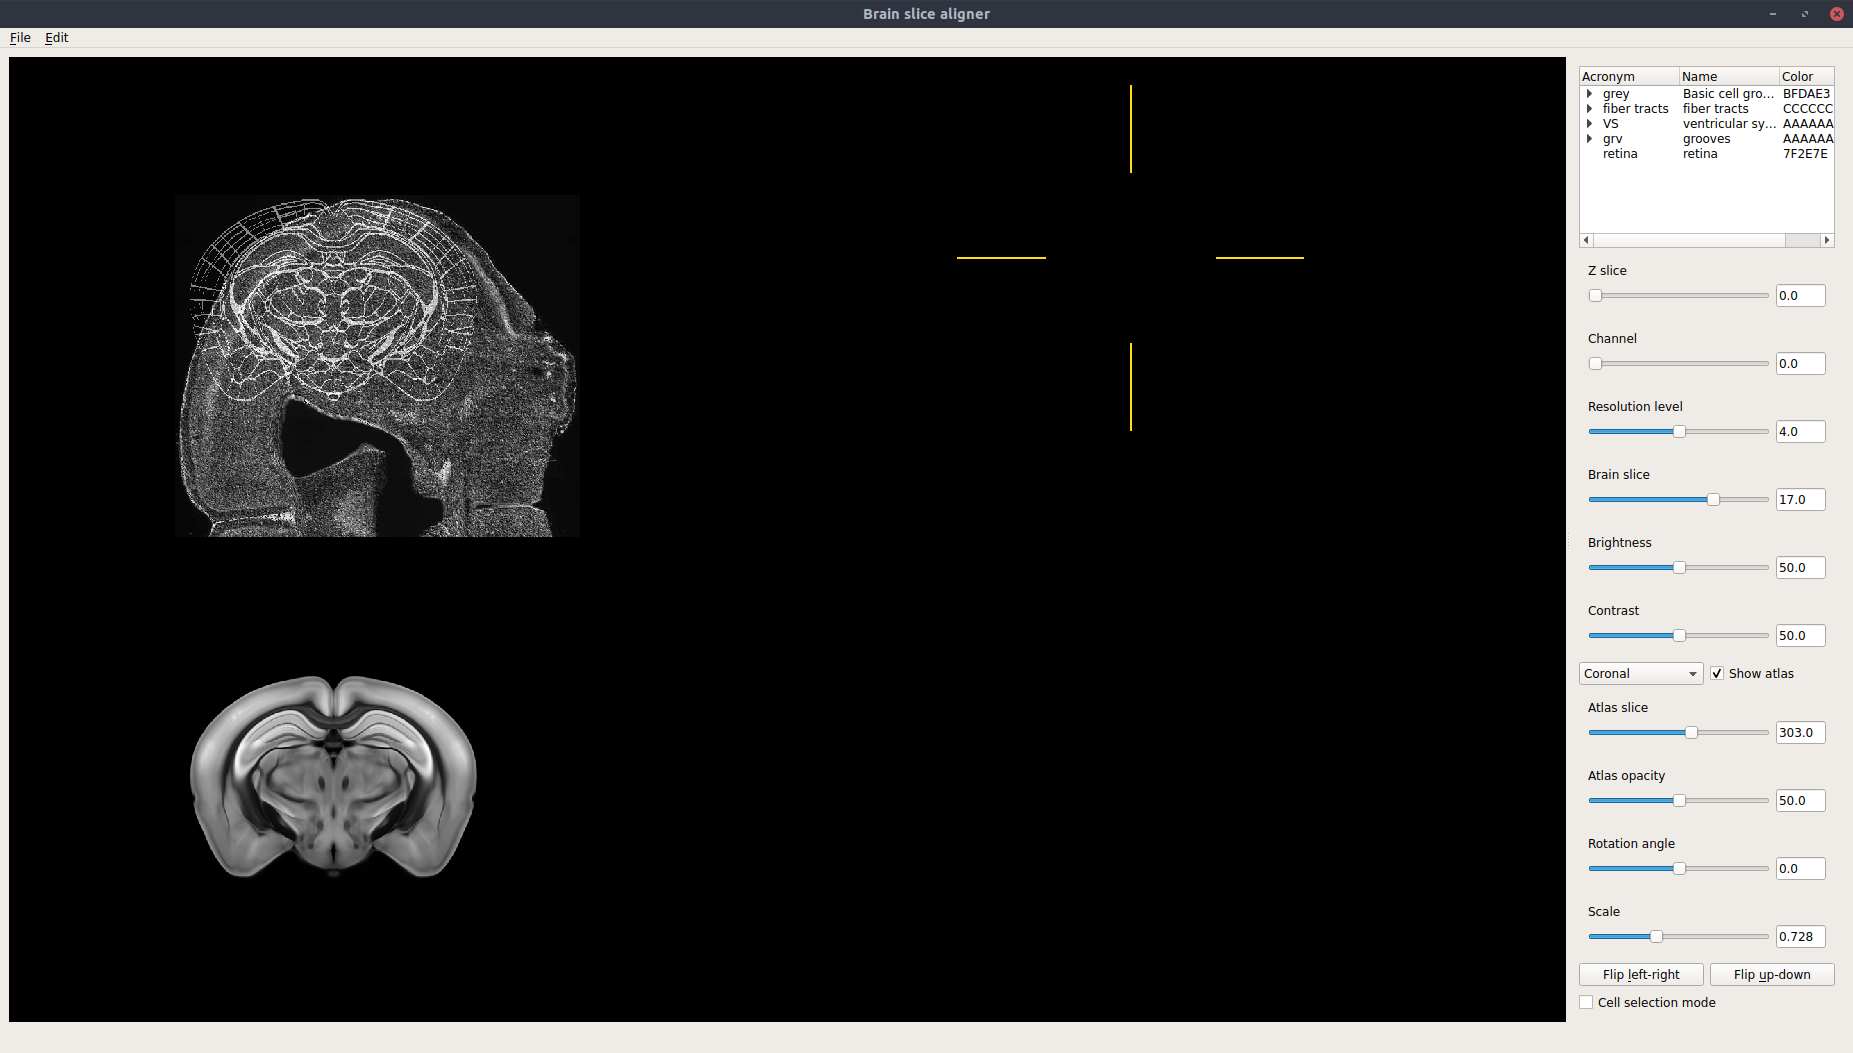
\includegraphics[scale=0.25]{oldWhenOpenImage.png}\\
\underline{Figure 1} : Screenshot showing the state of the software when opening an image \\ \vspace{1\baselineskip} \end{center}

\subsection{Graphic interface}
The main window is divided into four screens. The window on the left are used for viewing the atlas/image overlay. However, the 3D atlas displayed in the window at the bottom left is not used. The right part is used to select the points. The top window (right side) contains a copy of the opened image. This image is zoomed and is in its original quality. The two upper windows are synchronized: when the user wants to select areas of interest and browses the left image with the mouse, the right window allows him to preview the area. The cross visible in the figure below allows the user to point cells of interest (cf Figure 2).\\

Then, on the right side of the software, there is a side tab. It is first containing a box with the tree structure of the mouse brain. It's in the form of region levels, and each time the user clicks on a region, the daughter regions appear. Then, there are the different widgets allowing to carry out adjustments before use (adjustment of contrast, brightness, the opacity of the atlas) and during use (navigation in the slices of the atlas, activation of point selection mode). The user can also choose the section of the brain (sagittal, coronal or horizontal) that the atlas will take.\\

\begin{center} 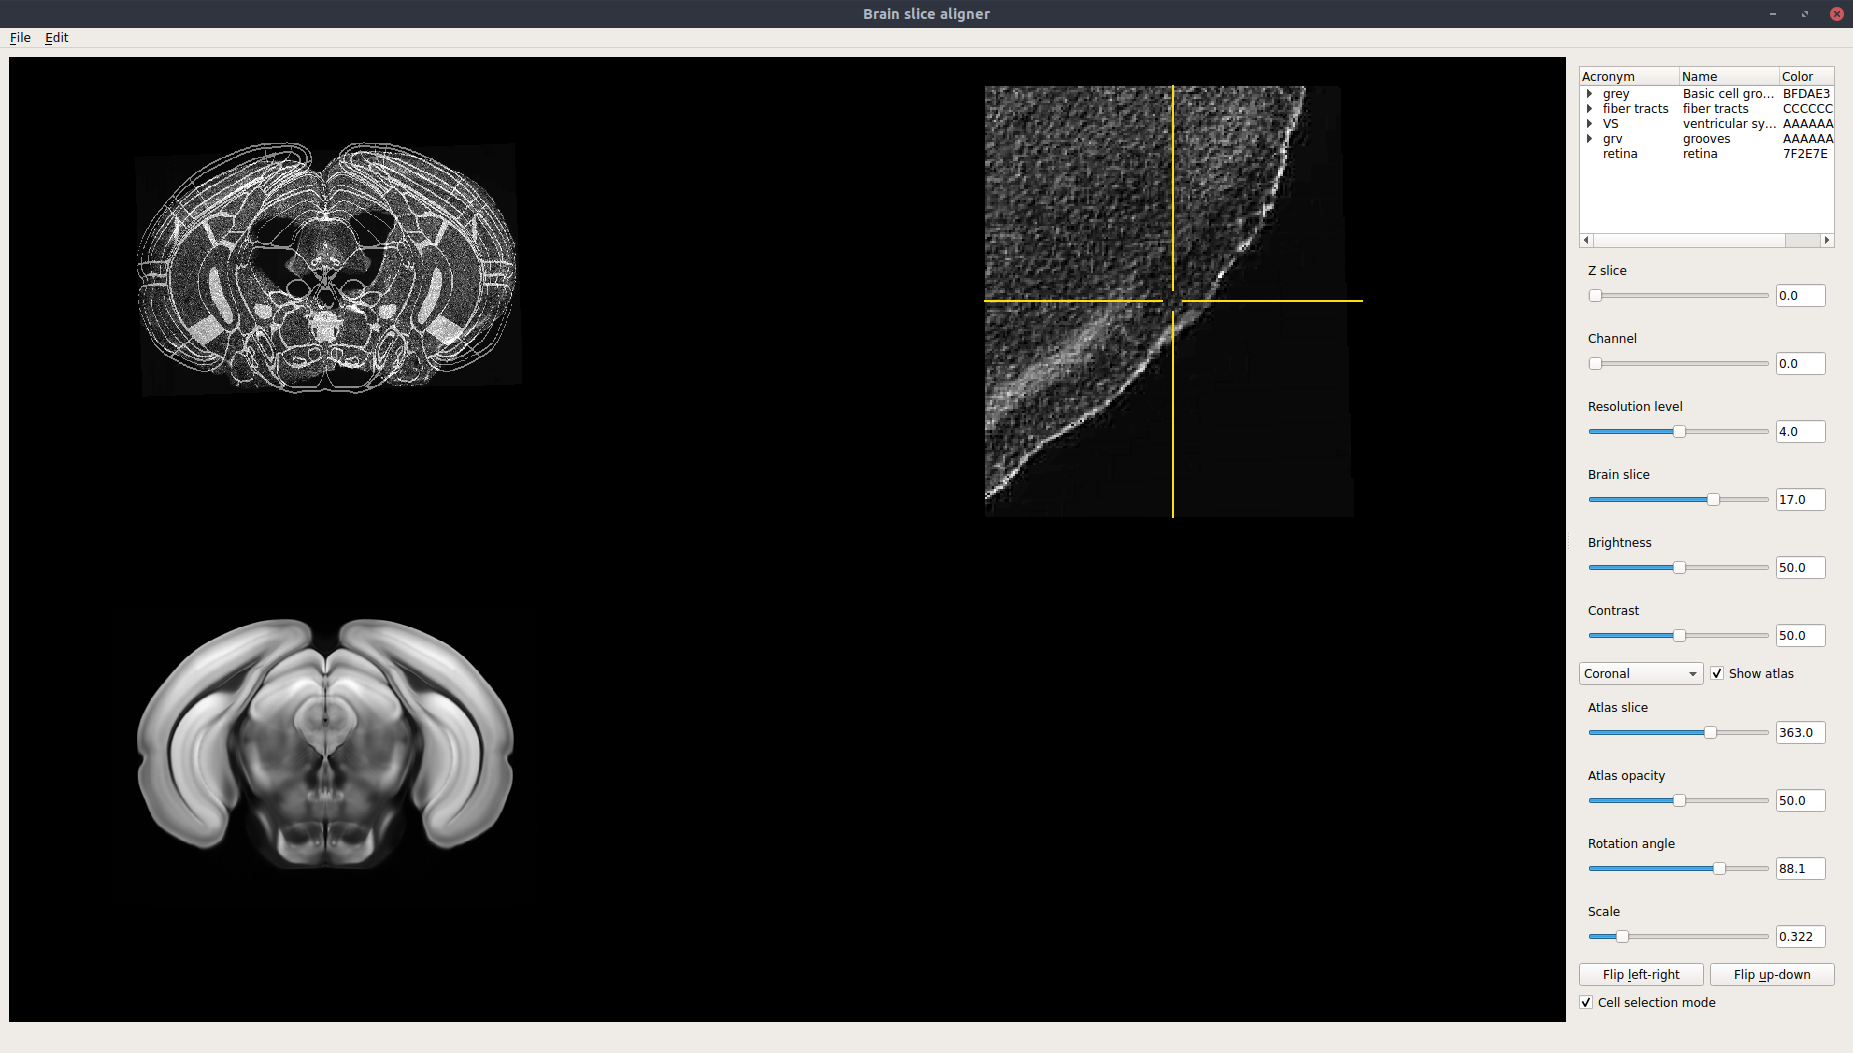
\includegraphics[scale=0.25]{oldWhenCellSelectionning.png}\\
\underline{Figure 2} : Screenshot showing the state of the software when the user is searching for areas of interest. The image was superimposed with the atlas manually. \\ \vspace{1\baselineskip} \end{center}

\subsection{Image handling}

All the images are acquired through an Hamamatsu NanoZoomer Digital slice scanner, providing whole slide images with different channels of fluorescence. Hamamatsu provides their customers with scanning and software solutions. The output format of images that comes from their whole slide scanner is NDPIS and Hamamatsu provides different softwares to open them. The NDPIS format allows to take several pictures of the same area, saved as NDPI images, for each fluorescence channel. These images are then linked by an NDPIS file. This linker allows the user to open images one by one or to superimpose them, as they are linked as images of the same region. NDPI images are basically images with a TIFF-like structure but can't be opened with the same tools as TIFF images : this is because TIFF format does not support files larger than 4 GB, but NDPI format can. \\

In our case, each NDPIS file link two NDPI images, one for the blue channel (DAPI) and one for the red channel (TRITC). Each one of these images contains several brain slices. As we need to align each slice with the atlas in the software, the user has to crop each brain slice from the NDPI image. From one NDPI image showing around ten brain slices, the user create around ten TIFF images showing one brain slice each. To do so, the user had to open each NDPI image with the NDP.View software provided by Hamamatsu. Then, on each image, select brain slices one by one with the "select region of interest tool" in NDP.View. Each region of interest was then saved as a JPEG image. This JPEG image was then converted to a TIFF image using a JavaScript script in ImageJ software. This conversion to TIFF image is mandatory as the Atlaser software can only open TIFF images. \\

\subsection{Main problems during use}
During the development of the software, several functionalities were implemented and commented out for certain reasons; the others are functional but pose a problem for the user. The current software allows us to view slices of mice brains and navigate between them. Currently, the user can select areas of interest by clicking on them, overlay it on a mouse brain atlas. During selecting points, when the image is superimposed on the atlas, the region where it is located is saved for each point. These data can be exported in the form of a spreadsheet.\\

\subsubsection{Image handling problems}
Regarding the NDPI images, the Atlaser software was providing tools to crop each brain slice and convert them into TIFF images directly using the NDPIS linker, cropping each brain slice from both NDPI images at the same time. The feature was not working well for two reasons : \begin{itemize}
    \item the user had to choose, through a slider in the software, which slide he wanted to crop and show on screen. When he was done with the first slice, switching to the second slice, the cropping process had to be done again to show the second slice on screen, forcing the software to open and process the whole slide image again;
    \item the user had to choose, through a slider in the software again, which quality he wanted to have for the final TIFF image shown on screen, resulting on the software having to process the whole slide image again.
\end{itemize}
The main reason this feature was not working well is the size of NDPI images. Each one of them is about 2 GB. Every time the user had to move a slider, the software was processing again two images weighting around 2 GB each. As a result, the tool could be used with low quality TIFF in output, or, then, we have TIFF images with a good quality, but it makes the software crashing.\\ 

\subsubsection{Superimposition problems}
The main feature of the software is to superimpose the brain image with an atlas. This allows the user to select cells and stock information about the location of this cell. The main issue was the number of steps the user had to go through to align the image and the atlas.
\begin{itemize}
    \item the image was neither opening with the same size nor the same orientation as the atlas, forcing the user to execute multiple changes of size and rotation on the image;
    \item it was difficult to move the image without moving the atlas, as most of the buttons and commands were moving both of them. The user had to change the scale of the image to give it the same size as the atlas, changing in the meantime the quality of the image.\\
\end{itemize}

\subsubsection{Luminosity problem}
When opening an image that was too dark on screen, the user can change the luminosity level of the image. The problem was that when moving, rotating or resizing the image, the luminosity was automatically reset at the minimum value, preventing the user from making multiple actions at a time. He had to change the luminosity after every steps when superimposing the image and the atlas. \\

\subsubsection{Points selection problem}
Once the image and atlas are superimposed, the user can click on neurons of interest to select them. Selected neurons can then be exported in an excel file with some information about each one of them. There was two problems with this feature :
\begin{itemize}
    \item the user could click multiple times on the same neuron, selecting it multiple times for the software but showing only one mark on screen. This was confusing as a neuron has no reason to be marked several times. The user could not see when it was the case, but if a neuron was selected tree times by error, the information about it were saved tree times in the excel file. 
    \item an other problem was that the user could not delete any random point he did. There was a "Delete point" command but only working for the last point. So if the user had to remove the point N-3, he had to delete the N-2, N-1 and N points first. \\
\end{itemize}

\subsubsection{Excel file output}
Once the user had selected all the neurons of interest, he could save the information about each neuron (position on the image, brain region) in an Excel file. There were two problems about this way of saving data :
\begin{itemize}
    \item Excel files are not the easiest to treat when generating or processing data, CSV format for example should be more adapted;
    \item in this file, only one brain region was saved when the user need to have more information about the location of each neuron, something more like a hierarchy of brain structures.  \\
\end{itemize}

\section{Functional and non-functional requirements}
\subsection{Ease while using the software}
\subsubsection{Graphic User Interface}
First of all, it is necessary to have greater visibility on the left part (image and atlas). Therefore, the 3D atlas present in the window at the bottom left has to be removed to give more space to the treated elements, that is to say, the brain slices and their analyzes with the atlas. The right part which corresponds to a zoom area (for a precise selection of points) will be placed in a corner to leave more room for the image and the atlas. Two additional elements discussed are the zoom and the selection: the zoom is not synchronized on the two windows, the cross which allows the selection is too large and the pointing area not precise enough. So, the two windows has to be synchronized while zooming. \\

Then, the selection cursor has to be modified for a better selection. Still concerning the selection of points, one of the problems encountered when saving data is that if the user clicked in the same place, each click is recorded (we can, consequently, have the same point many times). Also, the user cannot delete a click made: he must cancel all clicks until the one he want to delete. To overcome these two problems, the code has to be modified so that the same pixel can be selected several times but saved only once; by implementing a tool, it would be possible to delete any point, regardless of its position in the selection history. \\

\subsubsection{Image opened and atlas}
Currently, the atlas and images are fully synchronized in terms of movement, zoom and "click to determine the brain area". The problem is that the user can currently only modify the image via rotations and zooms, which causes problems when overlapping the two elements. It is important to be able to handle the atlas and the image separately. Consequently, tools (widgets or shortcuts) have to be implemented to give the user more ease during his work.\\

Finally, the buttons managing the contrast and brightness of open images have defects: resetting the modification (of contrast or brightness) when doing certain actions, etc... These problems have to be corrected. \\

\subsubsection{Image processing}
First of all, with regard to TIFF images, the sharpness of the image once opened has to be improved. Indeed, the images lose resolution when opening. A compromise between quality and ease of use will have to be found. \\

Now, regarding the NDPI images: the software was providing tools to open them and extract each brain slice as a TIFF image, but for this tool to work, the user had to sacrifice the quality of the output TIFF image. This is why they were using other software, like NDP.View and ImageJ, to extract each brain slice in a good enough quality and convert them to TIFF.\\

\subsection{Other software enhancements}
We think it would be interesting to be able to separate the two colors of the image (having a TIFF image with the red marker and a TIFF image with the blue marker) in order to be able to analyze the two.\\

Next, we would like to create a help tab where the user can easily access the various commands or shortcuts if he needs to. The addition of a guide to allow the user to have access to the different shortcuts can be created.\\

Also, we find it advisable to add more details when identifying the selected area of the brain. Currently, only the smallest sub-area is displayed; we would like to modify this so that the user can have at least three levels of hierarchies.\\


\chapter{Conception}{\setcounter{tocdepth}{1}} 
\section{Programming language}
The Atlaser project was developed using the Python programming language. It has high-level data structures and allows a simple but effective approach to object-oriented programming. Because its syntax is elegant, its typing is dynamic and it is interpreted, Python is an ideal language for scripting and rapid development of applications in many fields and on most platforms. The Python interpreter and its large standard library are freely available, in the form of sources or binaries, for all major platforms from the Python website \cite{python} and can be freely redistributed.\\

\section{Libraries, modules, and packages}
In this part, we will be interested in the different libraries, modules and packages which allowed to develop Atlaser software. First we will see how the GUI is created then all the image enhancement and opening part, in the same way for the creation of an atlas. Finally, we will see any widgets present in the application when using it.\\

\subsection{Graphic User Interface}
\subsubsection{Design and creation of a GUI}
To design the graphical user interface part of the Atlaser application, we used the PyQt5 library. PyQt is a module that allows to link the Python language with the Qt library and to create graphical interfaces in python. We use 3 modules in particular in this library:
\vspace{0.5\baselineskip}
\begin{itemize}
    \item \textbf{QtCore} : it contains all the essential and multiplatform classes that form the backbone of any PyQt application. They range from strings to process, input and output management, as well as various data structures.
    \vspace{0.5\baselineskip}
    \item \textbf{QtGui} : it contains all the GUI elements provided by Qt, from a simple label to the complex graphic view. All GUI elements in PyQt are called "widgets".
    \vspace{0.5\baselineskip}
    \item \textbf{QtWidgets} : this module provides the basic capability to render to the screen, and to handle user input events.\\
\end{itemize}

\subsection{Addition of analysis elements in the GUI}
The pyqtgraph library is a pure-python graphics and GUI library built on PyQt4 / PySide and NumPy. It is intended for use in mathematics / scientific / engineering applications. It is used to integrate elements into the graphic interface, such as the image at opening or the atlas. The two key points of this library are that it's provide fast interactive graphics for data display and tools to aid in rapid application development. \\

\subsection{Image processing and atlas creation with Python}
Images are handled through different libraries in the software :
\vspace{0.5\baselineskip}
\begin{itemize}
    \item \textbf{PIL} : The Python Image Library adds image processing capabilities to the Python interpreter. This library provides tools to process and manipulate various types of images.
    \vspace{0.05\baselineskip}
    \item \textbf{OpenSlide Python} : OpenSlide was first a C library providing an interface to read whole-slide images, which are high-resolution images used in digital pathology. In our case, OpenSlide provides tools to open images that come from Hamamatsu products.
    \vspace{0.5\baselineskip}
    \item \textbf{NumPy} : NumPy is the fundamental package for scientific computing with Python. In our case, it provides tools to convert images to N-dimensionnal arrays object. Working with such arrays allows us to apply mathematical transformation on pixels values with ease. 
    \vspace{0.5\baselineskip}
    \item \textbf{CV2} : CV2 (that comes from OpenCV) is a library to open, save and display images.
    \vspace{0.5\baselineskip}
    \item \textbf{Scikit-image} : Scikit-image is a collection of algorithms for image processing. It provides us morphological operations such as erosion or dilation.\\
\end{itemize}

\subsection{Python Standard Library}
\subsubsection{CSV}
CSV (Comma Separated Values) format being the most common import and export format for spreadsheets and databases, the CSV of the Python Standard Library is imported in order to manage the results.

\subsubsection{Collections}
The Collections library is used to create dictionaries storing strings when saving data at the end of use. \\
\subsubsection{sys Module}
This module provides access to some variables used or maintained by the interpreter and to functions that interact strongly with the interpreter. We use it for launching, closing and error handling software. \\

\subsubsection{Logging}
Logging is used to indicate that certain have occurred, displaying a message, some data or a variable.
Here, we used the logging module to display error messages when using the software and when developing functions.\\

\section{Inputs}
As an input, the Atlaser software can treat with TIFF and NDPIS images. TIFF images are very popular in image processing as they are very flexible file format for handling images and data within a single line file. On the other hand, NDPI are quite a bit complicated to work with. As we saw in section \textbf{1.3.4}, NDPI images are linked in an NDPIS file. This file often link several images together. In our case, these images are from fluorescence microscopy and weight about 2 GB.

\section{Outputs}
When the selection of points is finished, they are saved and an Excel file containing two sheets is obtained (cf Figure 3). The first contains the names of the regions and the number of times each region has been selected. The second sheet has five columns: the first indicates the coordinates of the point on the image, the second contains the name of the region, the third and the fourth are the coordinates again (x then y) and the fifth contains the number of times that we clicked on a pixel (value always equal to 1 even if we clicked several times). The export is carried out with the Pandas module. The \textbf{ExcelWriter()} method makes it possible to write the information in the Excel file, after having converted the attribute of the class which contained this information into a DataFrame (thanks to the Pandas library).\\

\begin{center} 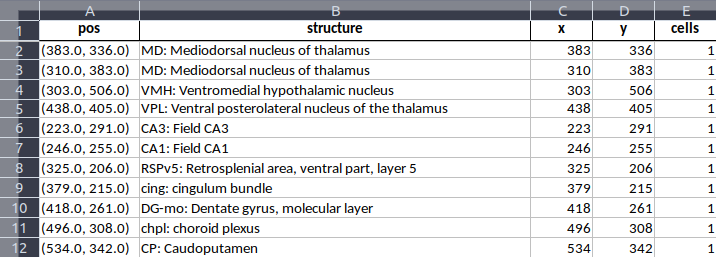
\includegraphics[scale=0.55]{excelOutput.png}\\
\underline{Figure 3} : Extract of open data in word processing software \vspace{1\baselineskip}\\ \end{center}

To allow the use of the text file obtained on different operating systems, we have modified the export format to CSV to make it easier. Dr. Frick being only interested in the selected region and its tree structure, this file now contains a single page with the coordinates and three columns corresponding to the selected region and its "parent" regions (the last two).\\

\section{Software architecture and quantification of work}
The four files contain 3703 lines of code in total (cf Figure 4). These 3703 lines allow the existence of 9 classes containing a total of 130 methods. There are also 29 independent functions. The existing classes correspond to objects, which once assembled, make it possible to constitute the software: buttons, windows, actions on the image (rotation, size management, ...), etc.... The architecture and composition of the classes is available in the appendices (cf Figure 15).\\
\begin{center} 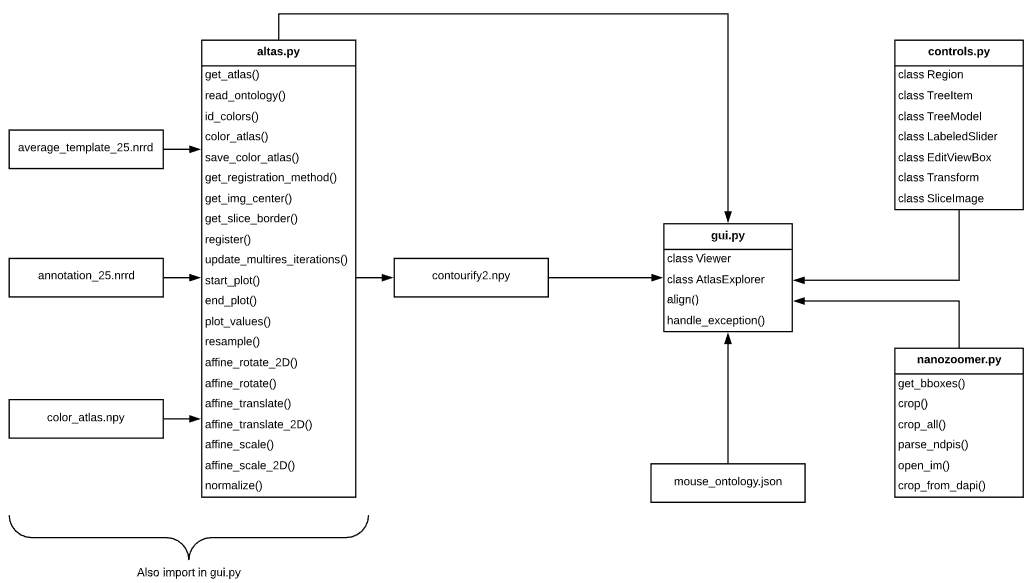
\includegraphics[scale=0.37]{filesBefore.png}


\underline{Figure 4} : Diagram representing the different interlinked files of the program before modifications.\\ \vspace{1\baselineskip} \end{center}

So, before starting our work, a repeated and precise reading of the code was carried out to understand how the elements were arranged, to understand the functioning of the classes and their methods and the bibliographic research on the various libraries used in particular in graphic development and image processing was performed. \\

At the end of reading the code, we estimated that we should touch around 500 lines of code or 15\% of the code (without counting the elements that must be added). Then, once the code has been understood and analyzed, we have deleted unnecessary lines to the version that we intended to offer to the customer to simplify the files in terms of content. Relationships between classes and between files remain unchanged. In summary, the software architecture has remained the same, the code has been reduced and the necessary elements have been added (cf Figure 5).\\ 

\begin{center} 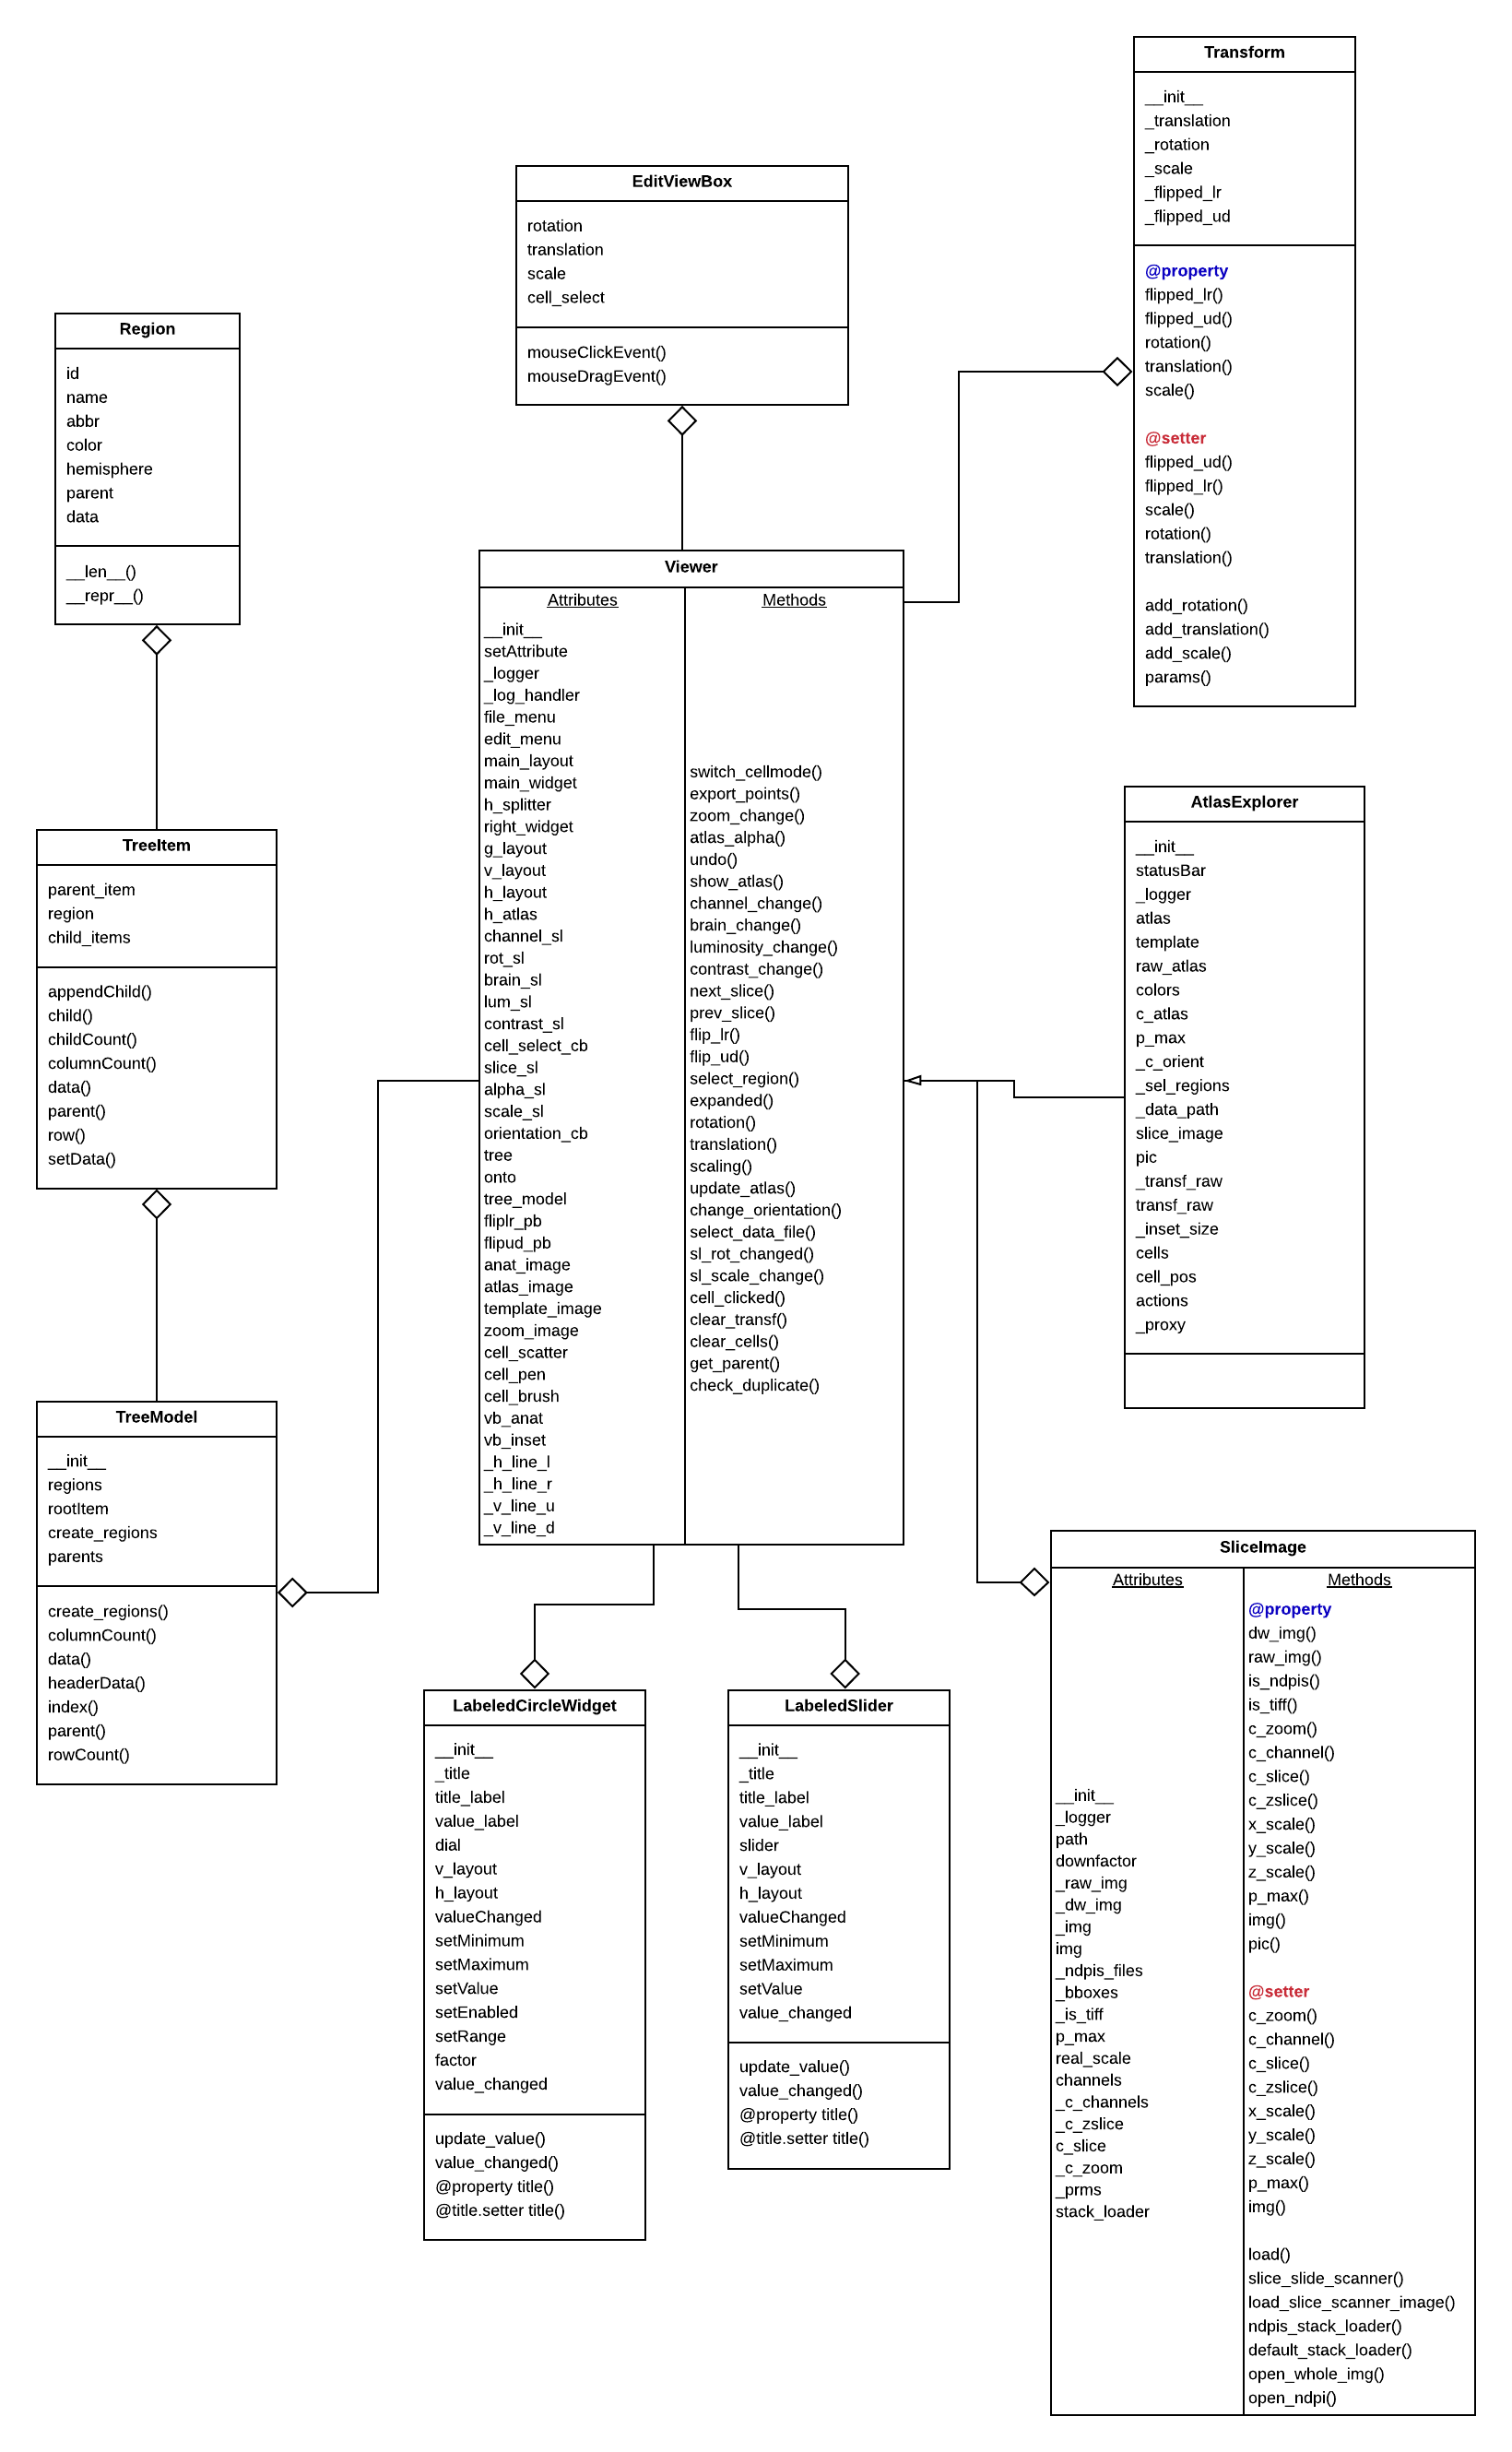
\includegraphics[scale=0.23]{newClasses.png} \\ 
\underline{Figure 5} : Class Diagram of the software presented in this document (after our modifications)

(\textit{as said before, the old class architecture is available in the appendix}).\\ \vspace{1\baselineskip} \end{center}

\chapter{Implementation}
\begin{center} 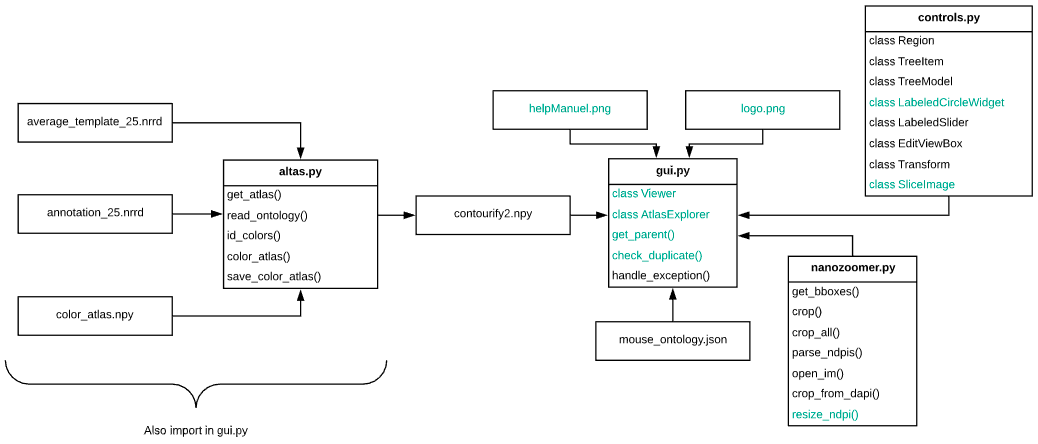
\includegraphics[scale=0.46]{newArchitecture.png}
\textcolor{white}{ouiouioui} \\
\underline{Figure 6} : Diagrams representing the different interlinked files of the program and the corresponding classes and functions (in green, new or modified elements regarding \textbf{1.4} diagram)\end{center}

\section{Graphic User Interface}
\subsection{Removing unnecessary windows}
The \textbf{Viewer} class is used to create the main window. One of its attributes is \textbf{main\_widget}: it is the main widget, i.e the black screen of the software. The geometry of this widget was modified using the \textbf{setGeometry()} method. This method takes in parameters four elements: X coordinate, Y coordinate, the width of the frame, the height of the frame. Finally, this window is placed in the center of the screen using the \textbf{setCentralWidget()} method applied to the Viewer instance. \\

Then, the 3D atlas present in the window at the bottom right was deleted(\textbf{vb\_atlas} attribute, methods, and functions that called it). In order to split the screen in two, we adjusted the \textbf{g\_layout} attribute: it is the attribute that stores the main widget. We have promote the GraphicsLayoutWidget instance (g\_layout) and add the items with code. This was done during the initialization of the \textbf{g\_layout} attribute: it was placed in argument of \textbf{GraphicsLayoutWidget()} the attribute \textbf{main\_widget}. This being done, we modified the geometry of this central window when adding the three elements (atlas, image, and image zoomed to the right).\\

The two windows stored in \textbf{g\_layout} are instances of the already existing \textbf{EditViewBox} class. It's a box that allows internal scaling/panning of children by mouse drag. It can be added ImageItem type objects (which is the case for the three elements to add). The two windows are added to \textbf{g\_layout} by the \textbf{addItem()} method which takes as argument a ViewBox object and the column and row number. In our case, \textbf{vb\_anat} (left window) is located at line 0, column 0 and \textbf{vb\_inset} (right window) at line 0, column 1. The atlas, image, and zoomed image are added to their respective ViewBox by the \textbf{addItem()} method also.\\

\begin{center} 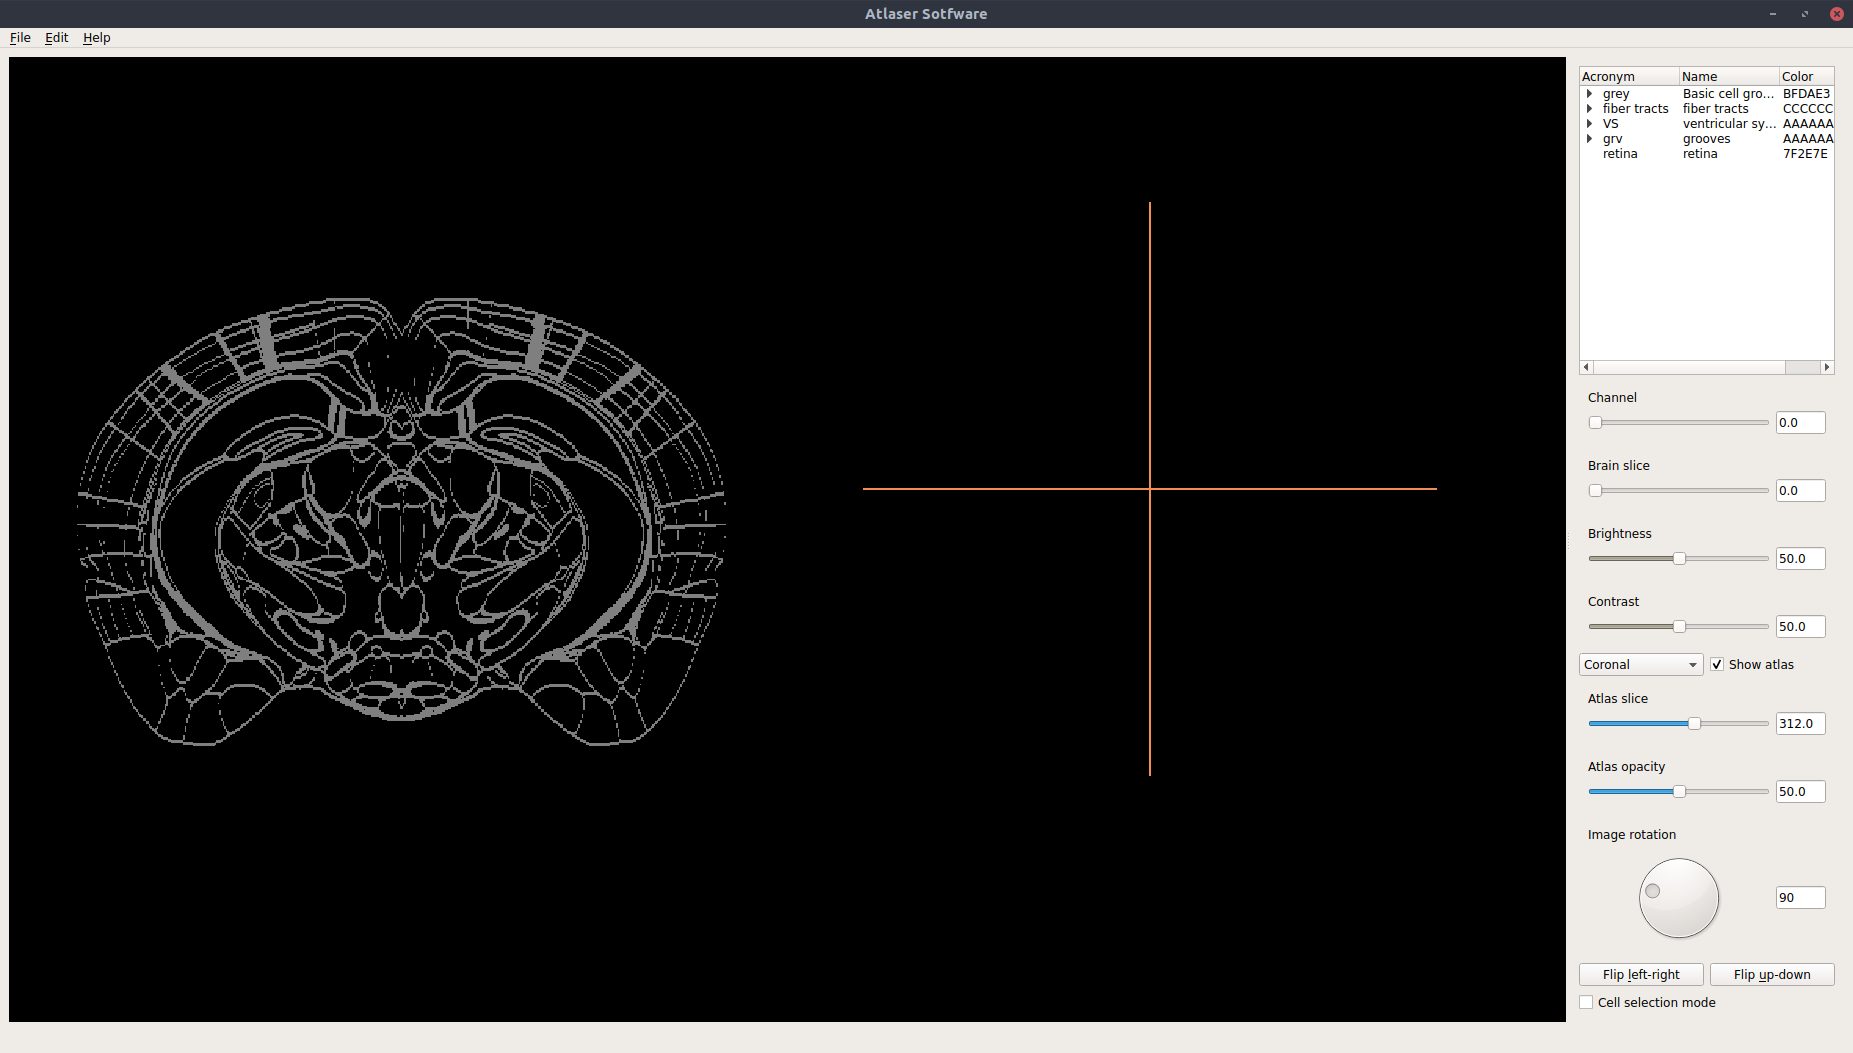
\includegraphics[scale=0.22]{newOpenSoftware.png}\\
\underline{Figure 7} : Screenshot showing the state of the software when the user launches it. \vspace{1\baselineskip}\\ \end{center}

\subsection{Improving the workspace}
Next, we wanted to improve the size of the user's work area (cf Figure 7). Indeed, by increasing either the size of the image or that of the atlas, it becomes possible to work directly on a single window, and thus it is possible to delete the right window used for selection.\\
\subsubsection{Increasing the size of the atlas}
First, the choice was to increase the size of the atlas and keep the native size (and thus the resolution) of the image. Opened TIFF images are large images with a high resolution. To keep these characteristics during the use, we have enlarged the atlas so that it has the same size as the image. Consequently, the user does not have to lower the size of the image, which would, therefore, allow having an image of very good quality.\\

First, the right windows was removed. For this, we deleted the \textbf{vb\_inset} attribute and all the functions that used it. Once this was done, we increased the size of the atlas so that it is the same size as a TIFF image when opened. The attribute used to display the atlas stores numpy arrays. So, we zoomed in on the image stored in these arrays of numbers using the \textbf{scale()} method. This method takes as argument two values and increases in width and length the image from the numpy array according to these values. However, this does not increase the active click area, as visible below: the circles can only appear in the old area where the atlas was before zooming (upper left) (cf Figure 8).\\
\begin{center} 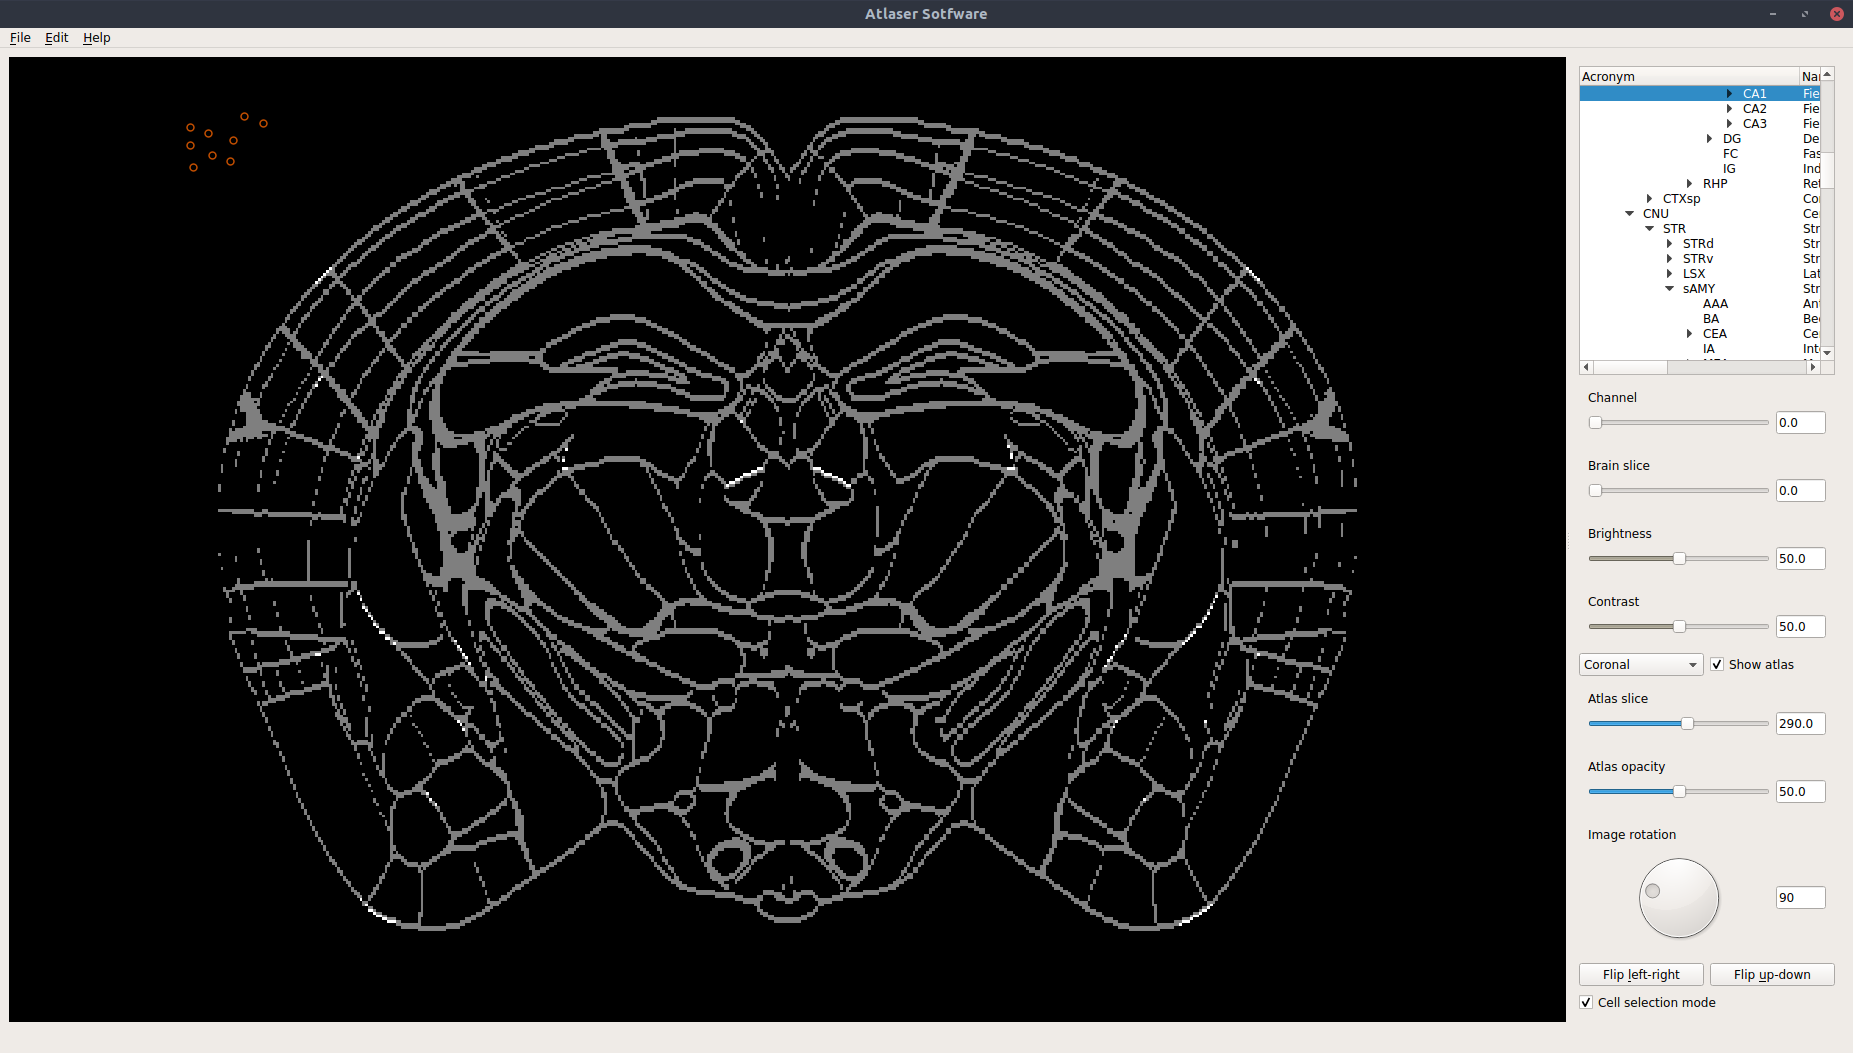
\includegraphics[scale=0.22]{bigAtlasBugSelec.png}\\
\underline{Figure 8} : Screenshot showing the state of the software with one window and only the atlas zoomed. \vspace{1\baselineskip}\\ \end{center}

We then modify the size of the coordinates retrieved in the \textbf{cell\_clicked()} method. It allows obtaining the coordinates of a click, retrieve the selected region, and draw a point on the clicked location. The values used for drawing the point (x and y) have been multiplied by 10 as well as the values stored in the cells dictionary used to save the data. After this, the points appear in the atlas. The problem with this modification is that now it is big area of 10 x 10 pixels that are recognized. If we click in this area, the same pixel is always recognized. This causes a big difference between the position of the click and the spot where the circle is drawn.\\

\subsubsection{Setting the image resolution value on opening}
Therefore, we changed our strategy following this, the aim being always to allow the user to have the least to do when opening the image so that he can quickly process an image. Thus, it is now the size and resolution of the images that have been changed. We removed the \textbf{scale()} method and removed the multiplication of coordinates. Knowing that all opened TIFF images have the same size (this is due to the acquisition software), we applied a down factor of 50 on the width and length of the image. This causes a loss of quality and detail on it, but when opened, it is aligned with the atlas and the two are the same size. To overcome this quality problem, we restored the right window. On this window is displayed the image in native quality, zoomed (display of 1000 pixels by 1000 pixels) on the area where the mouse is on the left window. We have modified the value of the \textbf{\_inset\_size} attribute accordingly and set it to 1000 (\textbf{Viewer class}). The result is visible below (cf Figure 9):

\begin{center} 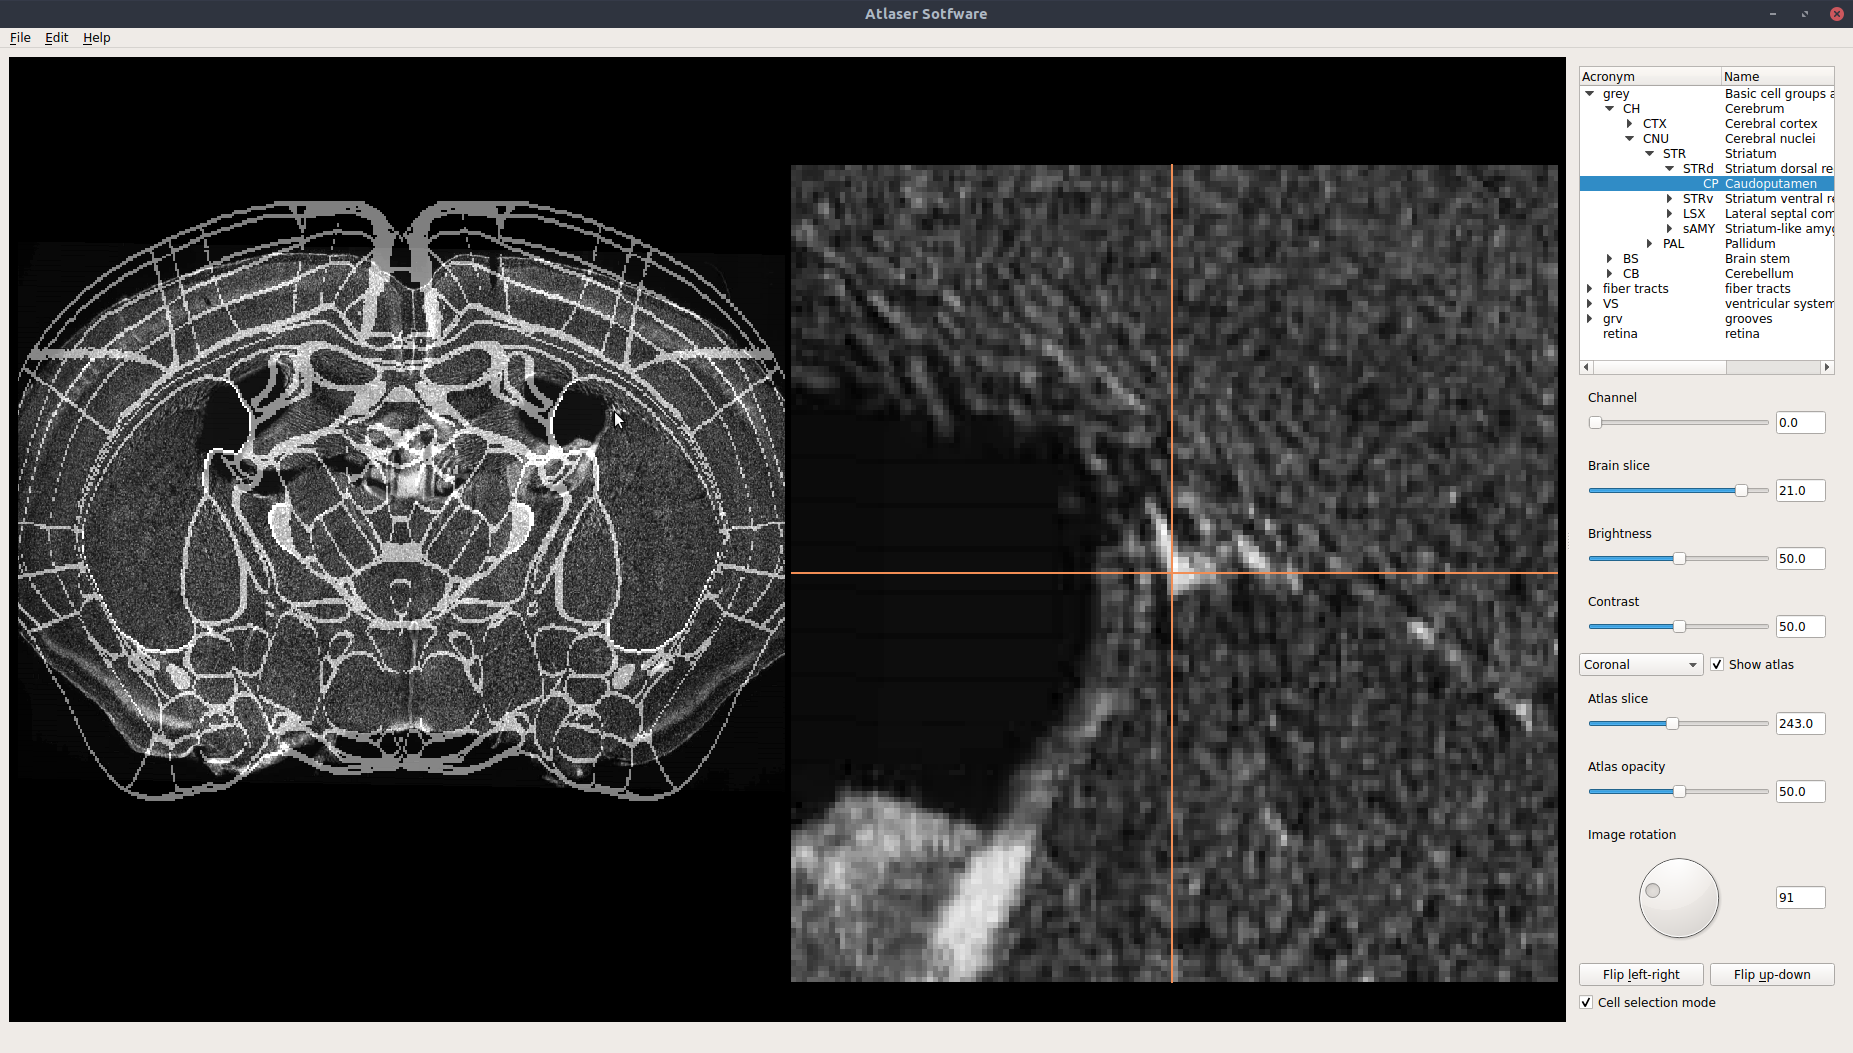
\includegraphics[scale=0.22]{finalVersionUsingSoftware.png}\\
\underline{Figure 9} : Screenshot showing the state of the software when doing region selection. \vspace{1\baselineskip}\\ \end{center}

Other improvements have been made: the cross is now a more thin and precise. The color of the cross and the selection circles are now more visible. \\

\section{Shortcuts, widgets and tabs}
\subsection{Shortcuts}
\subsubsection{Rotating, moving and scaling the image}
As described above, the already existing class \textbf{EditViewBox} allows to create an interactive workspace, that is to say that the user can move, zoom, or even click on elements of the window. It has four attributes that correspond to the actions that can be performed: rotation, translation, scale, and cell\_select. These four attributes are objects of the \textbf{pyqtSignal} class from the QtCore module. They take as parameters one (rotation value for example) or several floats (translation needs two new coordinates). We have modified one of the two methods of the class, \textbf{mouseDragEvent()}, to add keyboard shortcuts.\\

From the documentation of the \textbf{Qt} class and the ProgrammCreek website \cite{programmercreek}, we have created three shortcuts for rotation, translation, and scale. For each type of action, we recover which modifier is clicked. A modifier is a particular key on the keyboard that changes the action of another key or the mouse when pressed. Typically, these are keyboard keys such as CTRL, Shift, Alt, etc. Let’s take the example of rotation. We decided that the rotation would be done by clicking on CTRL and moving the mouse in the direction of rotation. If the event retrieved is a modifier and is equal to the QtCore.Qt.ControlModifier event, then, when the rotation event is over, we recover the new value and apply it to the image. For the other two actions, we use the values of \textbf{x\_shift} and \textbf{y\_shift} to move or resize the image. These two values correspond to the difference from the last position of the mouse (retrieved with the \textbf{lastPos().x() or .y()} method which gives the last position of a QMouseEvent event corresponding to the interactions performed with the mouse (click or movement)) to the current position (retrieved with the \textbf{pos().x()} or \textbf{pos().y()} method).\\


\subsubsection{Atlas manipulation}
The existing slider for changing atlas sections only allows moving 3 by 3, which is not precise enough. We have added two keyboard shortcuts to allow slice by slice movement. The shortcuts created are accessible with the left and right arrows on the keyboard. The two shortcuts created are objects of the \textbf{QShortcut} class of the QtWidgets module (and are named \textbf{atlas\_fwd} and \textbf{atlas\_bck}). We set the corresponding key to the shortcut: for example for the right arrow, it is QtCore.Qt.Key\_Right. A second argument is fixed and it is the main window (\textbf{self.main\_widget}): this is where the shortcut is "activated". Finally, we link this tool to the action of changing the slice. For this, we use the \textbf{activated()} then \textbf{connect()} methods. The activated method "activates" the shortcut and the connect method links the action to the shortcut. We connect it to the existing \textbf{next\_slice()} method. This method increases by one the value of the active slice and thus allows the movement (idem for the other shortcut, there is a method \textbf{previous\_slice()}).\\


\subsection{Widgets}
\subsubsection{Image rotation tool}
The code of this class is taken from that of the already existing \textbf{LabeledSlider} class and has been modified to have a circular widget. The \textbf{LabeledCircleWidget} class is inherited from the \textbf{QWidgets} class of the QtWidgets module. An object created from it has three attributes: a title, a value, and a graphic element which is an object of \textbf{QDial} class. The \textbf{update\_value()} method is used to update the value (change of the rotation value). If the value indicated is a number between the possible values that the widget can take, then the image is rotated, otherwise, a \textit{ValueError} exception is raised to avoid a malfunction of the program. The \textbf{value\_changed()} method is a setter used to update the value on the screen. The \textbf{title()} method allows giving a name to the button created and displays it on the widget tab (cf Figure 10).\\
\begin{center} 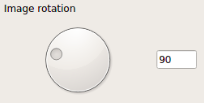
\includegraphics[scale=0.6]{rotationButton.png}\\
\underline{Figure 10} : Screenshot of the new rotation widget. \vspace{1\baselineskip}\\ \end{center}

\subsubsection{Removing unused widgets}
The buttons allowing to modify the slice on the depth, to change the channel, to modify the slice when using NDPI image, to change contrast value and the one to change the resolution of the image were removed because they are not necessary anymore. The first button does not work and is not necessary for the use of the client. The second is no longer necessary since the image resolution is now fixed at the opening. The associated attributes (\textbf{z\_sl}, \textbf{channel\_sl}, \textbf{brain\_sl}, \textbf{contrast} and \textbf{zoom\_sl}) and methods have been deleted from the \textbf{Viewer} and \textbf{AtlasViewer} classes.\\

\subsection{Removing unnecessary tabs}
In the tabs at the top of the software, it has been deleted various tabs that the user does not use: the one allowing to delete the modifications carried out on the image (rotation, size), the one allows saving a workspace and the one allowing to import one (that is to say import a list of points saved from a spreadsheet and display them on the screen).\\
\indent Also, the selection tool and the crop action not having been completed (see below), they are not available in the tab menu.\\

\section{Software tools}
\subsection{Exporting points selected in CSV format}
We have implemented a new \textbf{export\_points} method of the \textbf{AtlasViewer} class so that it can export data as a CSV file. First, we collect all the information about the clicks made. This data is stored using the cells attribute of the \textbf{AtlasViewer} class. This attribute contains a list and the information of each click is stored as a dictionary. We imported the \textbf{collections} module in order to create using the \textbf{defaultdict()} method, which allows us to convert the elements contained in the dictionaries of the cells attribute and to convert them to string in this new dictionary, in order to retrieve words not letters. 

Then, we define a path for saving the file. The file will be saved by default in the same folder as the one where the open image is. Finally, with the \textbf{csv} module, we use the \textbf{DictWriter()} and \textbf{writerows()} methods to write to the file. The \textbf{DictWriter()} method takes as argument the file, which we defined as \textit{open(path, 'a', newline = ' ')} and the dictionary keys (path corresponds to the defined path, 'a' allows write following an already existing file). The \textbf{writerows()} method takes the data as an argument, i.e. \textbf{self.cells} dictionnary.\\

\begin{center} 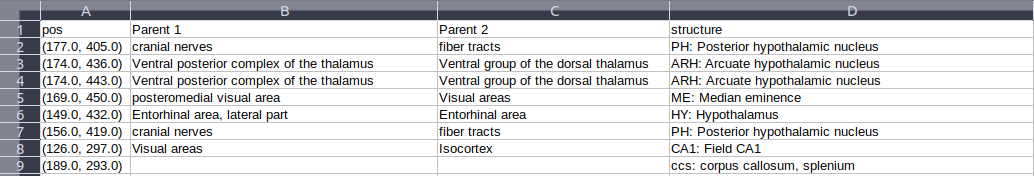
\includegraphics[scale=0.45]{newOutputCSV.png}\\
\underline{Figure 11} : Extract of the new format for saved data in a word processing software (LibreOffice spreadsheet) \vspace{1\baselineskip}\\ \end{center}

\subsection{Increasing the number of data saved}
When saving the data, the two parents of the zone having been selected are added to the spreadsheet in addition to the coordinates of the click and the name of the region. To make this possible, we created a \textbf{get\_parent()} function. This function takes as parameters a tree from a JSON file (here, attribute onto) and a target id. For each element of the tree, if the current element has the same id as the target id, we return this element; otherwise, we look at the child element of the current element, we apply the \textbf{get\_parent()} method to it and we add the element found in a list containing all the regions (from the first element to the child element searched). The elements are browsed from the top of the tree to his bottom to find the child with the target ID. The function is used in the \textbf{cell\_clicked()} method. We obtain the complete tree structure of the selected region and store it in the \textbf{cells} dictionary which will be exported. When saving, only the two closest parents (the last two before the selected region) are kept, as desired (cf Figure 11).\\

\subsection{Removing mistakenly selected points}
We have modified the already existing \textbf{cell\_clicked()} function, method allowing to click and draw, so that the user can now also delete points.

This action is carried out in the same way as for adding a point when selecting a region of interest thanks to the \textbf{cell\_clicked()} method. First, we get the coordinates of the current position with the function \textbf{convert\_mouse\_pos()}. This function returns the actual coordinates of the point: they correspond to the place where the user clicks on the screen; this is where the point is drawn. These coordinates collected are used to find the region of the atlas corresponding to the area clicked. When we know the area, we can get the name and id of the area. 

Then, the list of selected cells is added to the \textbf{cells} dictionary and this is what will be exported. At the end of the function, we added two controls (for loops): the first consists of removing duplicates from the window. Now, when the user clicks on a pixel, if the coordinates are already present in the \textbf{cells} dictionary, the point is deleted from the window. The second control is the removal of information from the dictionary. As before, if the information that should have been stored already exists, we delete this data. So, now, when we click on an existing circle, it is deleted and we delete the information of this point in the dictionary which will be exported later (cf Figure 12).
\begin{center} 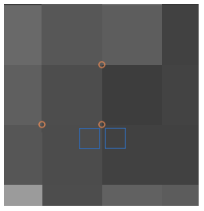
\includegraphics[scale=0.52]{deletePoints.png}

\underline{Figure 12} : Screenshot of active areas for deleting a point (the two blue squares are the areas to delete the point in the middle of the image) \vspace{1\baselineskip}\\ \end{center}


\subsection{Removing duplicates points}
We have implemented a \textbf{check\_duplicate()} function which removes duplicate selections. This method is used to delete the stored coordinates (dictionary \textbf{cells}) and the circles displayed on the screen (\textbf{cell\_scatter}) in duplicate. The method takes as argument a list (list 1). Another list is initialized (list 2). We start by browsing each element of list 1 and each time we browse the list 2. If the current element is not present in the list 2, then it is added to it. We end up returning list 2.\\

The \textbf{check\_duplicate()} function is used after adding the coordinates in the \textbf{cells} dictionary: we check that there are no duplicates when saving the clicked data. For the drawn circles, we use this function in the \textbf{undo()} method. This method initially made it possible to delete the last points recorded thanks to CTRL + Z. Now, since we can delete any point with the \textbf{cell\_clicked()} method (see above), we modified the method so that it traverses the dictionary containing the coordinates of the drawn circles (\textbf{cell\_scatter}) and removes duplicates. Thus, if the user clicks several times in the same place, the information is added and as long as he does not click elsewhere, the duplicates are stored. As soon as he clicks elsewhere, it removes duplicates. The shortcut CTRL + Z now removes duplicates (at the end of use for example, so as not to end up on storage of duplicates).\\

\subsection{Problems with luminosity and contrast}
The correction of the reset of the brightness when performing another action (use of another widget, change of slice of the atlas) has been corrected by adding to all the functions that control these widgets the following line: \textbf{self.apply\_brightness(self.lum\_sl.value())}.

This makes it possible to apply the active value of brightness after each use of another widget and thus not to reset it to 50.\\


\section{Image enhancement}
During this project, we tried to optimize the way image were processed. As we explain in section \textbf{1.4.1.3}, the user has to choose between using a TIFF image with a good quality, but coming from a long process, or opening an NDPI image to speed up the conversion between NDPI and TIFF, but obtaining images in low quality.\\

\subsection{Automated NDPI conversion}
To solve this issue, we implemented a feature to open an convert from NDPI to TIFF each brain slice automatically. To do so, we add the \textbf{open\_whole\_img()} function in the \textbf{controls.py} file. Previously, the software would not let the opening of NDPIS format, the aim of this function is to allow the user opening an NDPIS format, generating and saving brain slices from each NDPI image linked in the NDPIS file. There is tree major steps in this process : \vspace{0.2\baselineskip} 
\begin{itemize}
    \item First, we need to stock in the software the name of each image linked in the NDPIS file. In the \textbf{SliceImage} class in \textbf{controls.py}, we have the \textbf{\_prms{}} attribute. It is the dictionary used to stock the number of images and their name from the NDPIS file.
    \item Then we need to create directory to save the brain slices as TIFF format. We obtain two kind of slices : DAPI or TRITC. For each NDPIS file we open, if no directory has the same name as the NDPIS file, we create one with two sub-directories in it.
    \item Finally, for both DAPI and TRITC images, we use the \textbf{crop\_from\_dapi()} function from \textbf{nanozoomer.py} file to generate our brain slices.\\
\end{itemize}

\subsubsection{Image processing function in \textbf{nanozoomer.py}}
The \textbf{crop\_from\_dapi()} function is cropping each brain slices from both DAPI and TRITC images using bounding boxes.\\
\indent Bounding boxes are imaginary boxes used to demarcate objects in an image. To generate our bounding boxes, we use the \textbf{get\_bboxes()} function in \textbf{nanozoomer.py}. This function load the DAPI image containing all the brain slices and create a bounding box for each brain slice, using a combination of dilation, erosion and binary closing on the thresholded image. This process return a number of bounding boxes equal the number of brain slice on the DAPI image, each bounding box defined by the position of the top-left pixel, its width and height.\\
\indent Once we have our bounding boxes, the \textbf{crop()} and \textbf{crop\_all()} functions will use them to crop each brain slice from the base NDPI image. \\

At the end, the \textbf{crop\_from\_dapi()} function is using all the above functions, but will apply the same process for both DAPI and TRITC images, as they are exactly the same, just the color channel is different. \\

\subsubsection{Problems of the automated NDPI conversion}
This method is by far the best for the user, as he has nothing to do but open an NDPIS file and wait for the result. Unfortunately, the NDPI images are too heavy to be processed this way by a standard computer. The \textbf{crop\_from\_dapi()} function is using the \textbf{OpenSlide} library to open and crop images, as this library provide the \textbf{read\_region} method to define a region to read from a whole slide image. Given this method the image with all the brain slices and a bounding box, it will crop at the position of the bounding box. The problem is that using this \textbf{read\_region} method on DAPI and TRITC image, the computer has to process two images weighting around 2 GB each, and save around thirty TIFF images weighting 300 MB each. As soon as we start the process, the computer doesn't respond anymore, eventually crashing during the process. \\
\indent At this point, we chose to abandon this feature, and tried to find a way to avoid this problem. \\

\subsection{Using a region of interest tool to crop brain slices}
As our main goal is to ease the conversion process between NDPI and TIFF, we had to think how to create a tool to crop brain slices from the NDPI images and save them as TIFF without crashing the software. Right now, as we explain in section \textbf{1.3.4}, the user need to crop each brain slice using the NDP.View software and then convert the output image to TIFF using ImageJ. To solve the issue of having to switch between softwares, we implement a select Region Of Interest (ROI) tool. The goal is to let the user select the region he wants to crop directly from the NDPI image containing all the brain slices and save it as a TIFF. The process will then be the same as using NDP.View and ImageJ but it will be done directly in the Atlaser. \\
\indent The first step is to open and show on screen the image containing all the brain slices. To do so, the \textbf{resize\_ndpi()} function in \textbf{nanozoomer.py} is used to open an NDPI image and save as TIFF a downscale version of it. We are forced to downscale the image of at least a factor 8 or it won't be shown on screen as the source NDPI is too big. Loading it with the \textbf{OpenSlide} library is possible but to display it we need to use the \textbf{PIL} library, which can't open image bigger than 178,956,970 pixels, even when \textit{Image.MAX\_IMAGE\_PIXELS = None} is specified. Once the TIFF image is saved, the user can open it in the software. \\
\indent To select the brain slices the user wants to crop, we created a selection tool using the \textbf{PyQtgraph} library (cf Figure 13). To use it, the user have to open an image and then click on "selection tool" in the "edit" menu. This action will make a rectangle appear on the image. This rectangle can be moved and modified in size, to fit the area the user wants to select. This tool is define in the \textbf{AtlasExplorer} class in the \textbf{gui.py} file, linked with the \textbf{update()} function.
The goal of this tool is to superimpose the rectangle with the brain slice to crop. Each time the user moves or changes the size of the rectangle, a list is updated that contains the bottom-left pixel's coordinate and the width and height of the region (cf Figure 16, appendices). This information will then be used to crop this region from the base NDPI image and not on the TIFF opened in the software, as the TIFF image is a downscale version of the NDPI one. 

\begin{center} 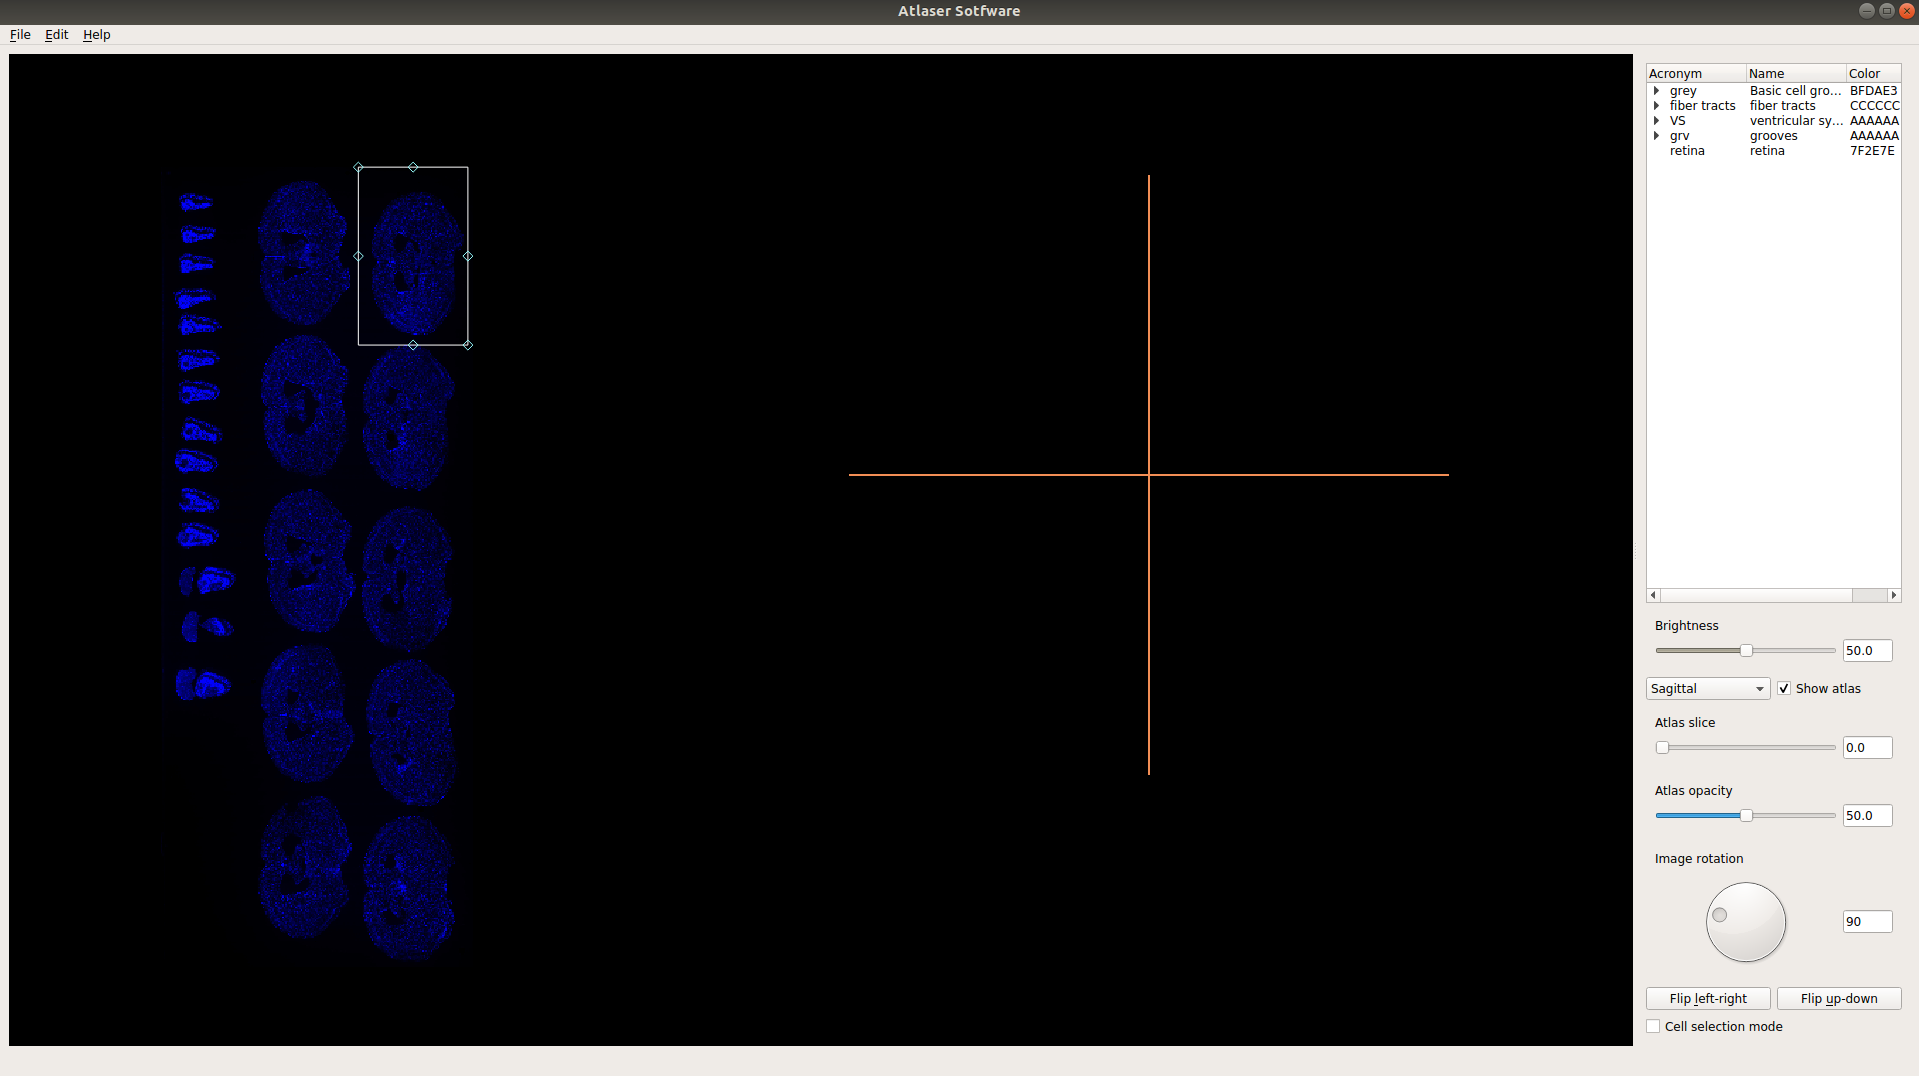
\includegraphics[scale=0.23]{ROITool.png}
\underline{Figure 13} : Screenshot of the window when opening an image in NDPI format (blue channel). The selection tool is visible in white. \vspace{1\baselineskip}
\end{center}


\subsubsection{Problems of the ROI tool}
This solution is the most flexible for the user, as he can chose to crop only some of the slices from the NDPI image, make the point selection and then go further. Unfortunately, we could not finish this feature in time, as there are still some problems to resolve :\vspace{0.2\baselineskip} 
\begin{itemize}
    \item First, the ROI selection is stocking information about the region to crop in a list using as a starting point the bottom-left pixel, but to crop from the NDPI image we need to use the \textbf{read\_region()} method from \textbf{OpenSlide} library. The problem is that this method is cropping using as a starting point the top-left pixel. 
    \item Then, the image displayed on screen is a down-scaled TIFF version of the NDPI image. When a region is selected on the TIFF image, the width and height of the region are not appropriate to crop on the NDPI image. This can be resolved by multiplying these values by the value of the downscale factor. The main issue comes from the coordinate of the bottom-left pixel, that can't be found using the same method of multiplying by the downscale factor. When down-scaling an image using the \textbf{read\_region()} method, the only pixel that keeps its coordinate is the top-left one (0,0). This second point make the first one even harder.
    \item Finally, for the user's quality of life, we need to crop in the exact same way the DAPI and TRITC images. When testing the automated cropping, we were using the NDPIS file as a linker, to keep in memory what are the two images to process simultaneously. In the case of the ROI selection, we are not opening the NDPIS file, only one of the NDPI image as a TIFF. Yet, we still need to crop both NDPI images (DAPI and TRITC) using the same ROI. We will need to find a way to apply this ROI on both NDPI images, given that the two first points are not problems anymore. \\
\end{itemize}


\section{Others changes and tools implemented}
\subsection{Help manual}
A Help tab is now available in the vertical tab bar. This is is an object of the \textbf{QMenu} class (of the QtWidgets module). The title of the tab is placed as a parameter and is followed by the object to which it belongs (here, \textbf{self}). Then, the \textbf{addAction()} method allows to create a new action with a text and a possible shortcut. In our case, when the user clicks on the Help tab, and then on the \textit{Manual} tab, it opens a PNG image. This image contains the various shortcuts described above. The user can also open this notice by performing CTRL + H. This is made possible by the \textbf{Qt} class of the QtCore module. The manual is visible in appendix (cf Figure 17). \\ 

\subsection{Software logo}
When the main program is launched, an icon appears on the computer icon bar. This logo was produced using the Canva website \cite{canva}. It's a free site, and the logo is copyright free (cf Figure 14). The \textbf{setWindowIcon()} method is applied to the main window which is an object of the \textbf{AtlasExplorer} class. In parameter is placed an object of the class \textbf{QIcon}.
\begin{center} 
\includegraphics[scale=0.40]{logo.png}\\
\underline{Figure 14} : Atlaser's logo. \vspace{1\baselineskip}\\ \end{center}

\section{Discussion and further developments}
As discussed multiple times along this report, the main focus was to improve the user's experience and to reduce the time processing each image.\\

First, we removed every features that were not used or non-functioning, improving the visibility and code clarity. At the end of the project, our code contain 3283 lines (from 3703), 10 classes (from 9) with 136 methods (from 130) and 17 independents functions (from 29).

Then, we fixed every problems that were slowing down the user when processing brain slices. The superimposition mechanism was too slow, as the user had to go through too many steps to have the atlas and the image aligned. To solve this, we created more shortcuts, we modified the user interface and changed the way the image is opened. Now, the image is almost superimposed with the atlas as we open them, both of them can be moved separately and there no more problem with the luminosity of the image.

When it comes to neurons selection, the brain slice image is now more visible on the left panel, the selection tool on the right panel shows in high quality a zoomed version of the image, allowing to make an easier selection. The zoom level on the right panel allows to see the region the user is in but is zoomed enough to distinguish different neurons.

The selection system was improved too, as each selection point is now unique an can be removed without loosing information on other points. Each of them, when exported, shows the user more information about the brain region that contains the neuron of interest.

Regarding the use of NDPI images, we tried all along the project to improve how the user can crop from them, first automatically and then with a new tool dedicated to it.\\

\subsection{More to do...}
More things could be one to fully optimize the Atlaser software. First, as we said previously, we could not provide a feature to treat NDPI images. The automated attempt is not the way to go, as a standard computer can't handle it. It could be interesting to go further with the development of the ROI tool as it is how the users are doing it right now but in an other software. An other solution could be to treat the image the same way Google Map is treating their images : the more zoomed the image is, the highest the quality. If so, using directly the NDPI image with all the brain slices could be an option, without having to crop them.

An other improvement would be to create an atlas with more information on it to be saved. For example, with the regions we could save the brain level (Coronal level 123) or the Bregma distance. These information are available on the Allen Brain Atlas website, but not on the JSON file we use in the software.

Finally, there are still some little bugs in the software that should be corrected, shown in the bugs report (cf. appendix).\\

\subsubsection{Atlaser dedicated to fluorescence}
During a meeting with Andreas Frick and his team to discuss the start of our work after validation of the specifications, he introduced us to a member of his laboratory and the fact that she also has images acquired in the same way as before. Nevertheless, she has a different need : she would like to have a tool allowing her to visualize the borders of the regions of the brain on her images (currently, she draws them manually on the image). Then, when the borders would be visible, she would like to be able to click on a region and be able to determine the level of fluorescence present on the selected region and, via a known formula, convert this luminosity into protein expression levels. The output file would also be a spreadsheet with the name of the region, the name of the protein used for labeling, and the protein expression value.

Since the software already has an atlas and a system allowing the user to select a region, we started to work on this version of the software when all the points mentioned in the specifications were finished and that the customer has validated these modifications.\\

We came with a slightly new interface derived from the Atlaser and started to implement the first features (cf Figure 18, appendices), unfortunately running out of time before having enough information on how the mathematical formula should work given the pixel intensity.\\

\chapter*{Conclusion}
\addcontentsline{toc}{chapter}{Conclusion}
As part of this project, a first version of the Atlaser software was developed by Dr. Frick and his team to analyze brain slices of mice using an Allen Institute atlas to identify the regions observed on the slices. This achievement allows us to deepen our knowledge of the neocortex, which is an important element in understanding some diseases such as autism. Even if this version of the software fulfilled the main objective, it remains nevertheless perfectible on some aspects.\\

We chose to integrate this project, within the framework of our UE Design of a Research and Development Project, because it is totally different in terms of approach and design compared to all of our projects carried out during the year. Indeed, we were able to develop and improve new skills throughout our collaboration with Dr. Frick and his team:\vspace{0.2\baselineskip} 
\begin{itemize}
    \item first of all, listening to our client’s needs in order to improve the use of the initial software. For this, a thorough understanding of the subject and the objectives to be achieved was the key points of this project;
    \item then, the part that was totally new to us and that motivated us to take this topic is the code review stage. By recovering the Atlaser software, it was necessary to dive into the program in order to understand its construction, the classes, methods used and their functioning to test the various problems and improve the operation of the software. It is this step that took us the longest because so far we have designed applications from scratch. So we had to learn the best practices methodically to perform a complete code review;
    \item finally, constant teamwork throughout the project is essential. Many exchanges are necessary with Dr. Frick and his team to better adjust the modifications made by us on the software as well as the additions of new features.
\end{itemize}
\vspace{0.2\baselineskip} 

\indent To conclude, our integration in this project was aimed at recovering the basic architecture of the Atlaser software and bringing new functionalities necessary to support Dr. Frick and his team in their various studies on the mechanisms of the cortical plasticity under normal and pathological conditions.

This requires a simpler and more adapted user experience, an improvement and the addition of new features allowing more precise control over the analyzed data and finally clearer results in order to recover the essential data. This update of the Atlaser program makes it possible to lose less time on the software, its use and therefore to focus as much as possible on data analysis which is essential on this type of subject.

\chapter*{Acknowledgements}
\addcontentsline{toc}{chapter}{Acknowledgements}

First, we would like to express our deepest appreciation to our client Dr. Andreas Frick for giving us the opportunity to work on this exciting project. Thanks to that, we have acquired essential
knowledge in code review, image exploration, graphical interface development and maintenance, object oriented programming and also the importance of the bibliographic part (library of modules, packages, etc.). We would also like to thanks his team who demonstrated flawless patience and who were most understanding and helpful throughout the project. \\

A special gratitude we dedicate to Dr. Marie Beurton-Aimar for guiding us through the process
of developing a professional project, for taking her time in order to bring us a most constructive and pragmatic outside look during each stage of this project, and this even despite this period of confinement. \\

Finally, we would like to thank Dr. Remi Proville for the advice he was able to give us and the tracks he suggested we study in order to obtain the best results during our project. \\

\bibliographystyle{unsrt}
\bibliography{sample.bib}

\addcontentsline{toc}{chapter}{Bibliography}
\printbibliography


\chapter*{Appendices}
\addcontentsline{toc}{chapter}{Appendices}


\begin{center} 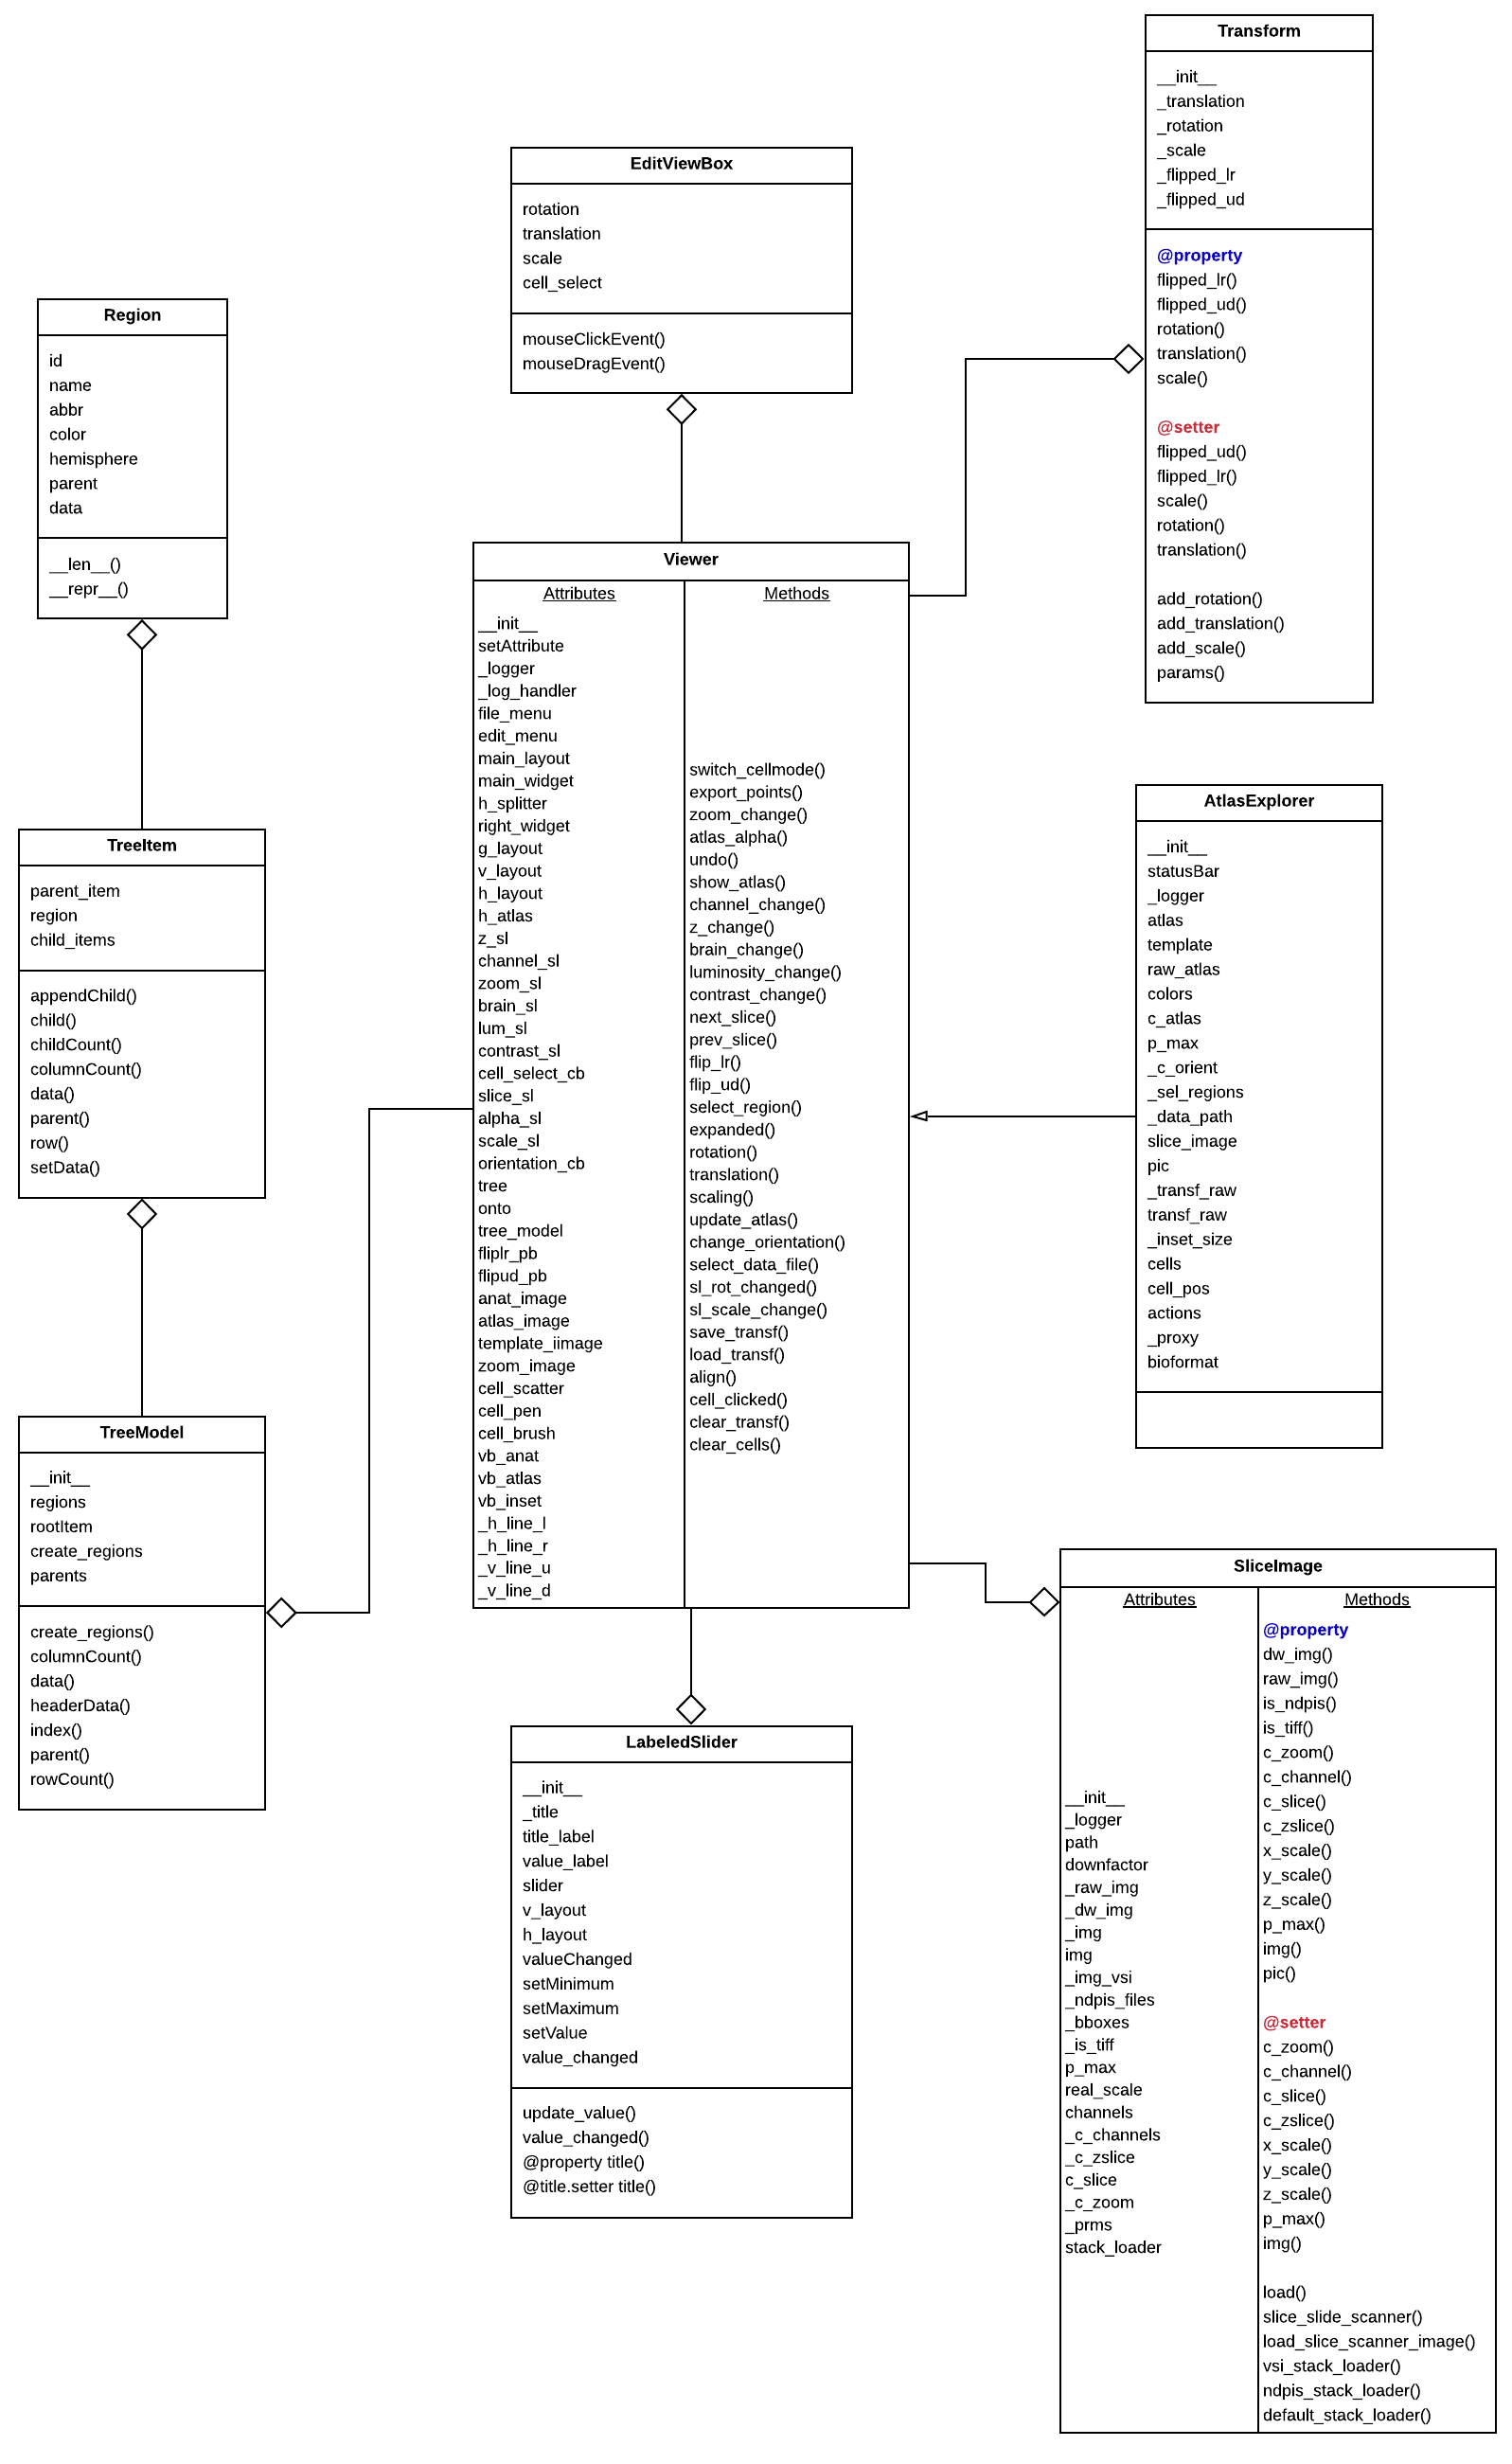
\includegraphics[scale=0.4]{oldArchitecture.png}

\underline{Figure 15} : Class Diagram of the software presented in this document (before our modifications). The diagramm echoes the one in part \textbf{2.5/ Software architecture and quantification of work} \\
\end{center}

\begin{center} 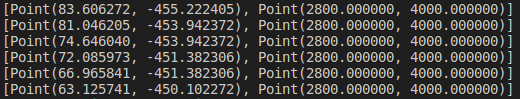
\includegraphics[scale=0.6]{coordinatesROI.png}

\underline{Figure 16} : Screenshot of the coordinates recorded when using the selection tool. These coordinates are visible in the log file or on the console. The screenshot echoes the image in part \textbf{3.4.2/ Using a region of interest tool to crop brain slices} \\
\end{center}

\textcolor{white}{ouiouioui} \\
\textcolor{white}{ouiouioui} \\

\begin{center} 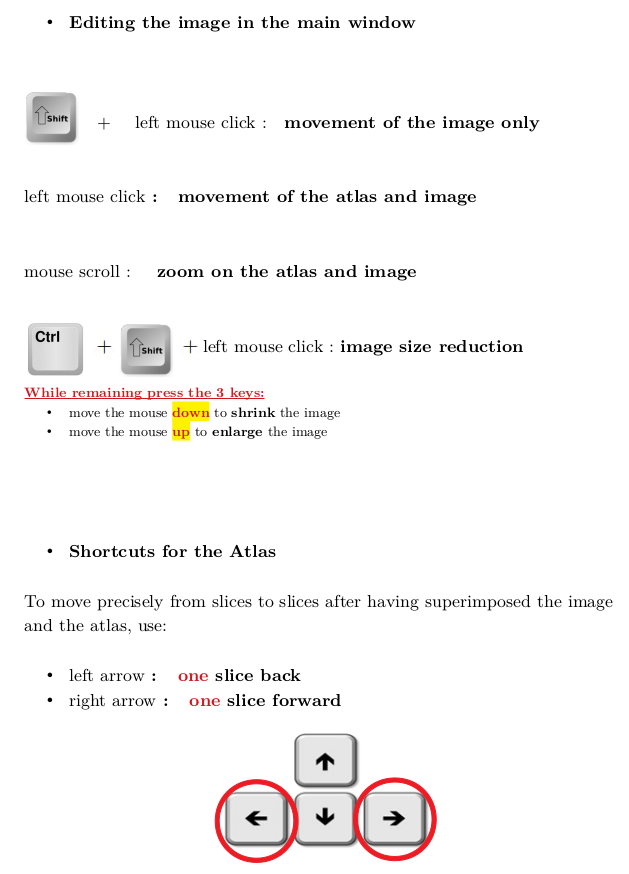
\includegraphics[scale=0.5]{helpManuel.png}

\underline{Figure 17} : Help manual \\
\end{center}

\newpage

\begin{customFrame}
import csv
import math

def openData():
    """ Opens a CSV file and return a dictionnary of proteins data. 
    First column = proteine name
    Second column = Sa value
    Third column = Kd value
    Fourth column = L value
    Each line = a protein with four informations about it """

    reader = csv.reader(open('protein_data.csv'))
    dataProtein = {}
    next(reader)
    for row in reader:
        key = row[0]
        if key in dataProtein:
            pass
        dataProtein[key] = float(row[1]), float(row[2]), float(row[3])
    return dataProtein



def applyFormula(data, key):
    """ Dans le fichier gui, quand on appellera la fonction, 
        il faudra bien voir qui est data. Puis, il faudra lier le choix
        actif sur le menu déroulant à key, pour qu'à chaque changement,
        il y est mise à jour 
        
        Takes as argument a dictionnary (data) and a key (name of the protein) and return the value C"""

    C = (1/data[key][0]) * ((data[key][1] + data[key][2]) / data[key][2])
    return C


data = openData()
C = applyFormula(data, 'musc')
C1 = applyFormula(data, 'rx82')
C2 = applyFormula(data, 'ly34')
print("")
print('FORMULA','\n(1/Sa) * ((Kd + L)/L)', '\n')
print("C :", C)
print("C1 :", C1)
print("C2 :", C2)\end{customFrame}
\begin{center} \underline{Figure 18} : Script containing the coded functions for the fluorescence version \end{center} \vspace{1\baselineskip} 

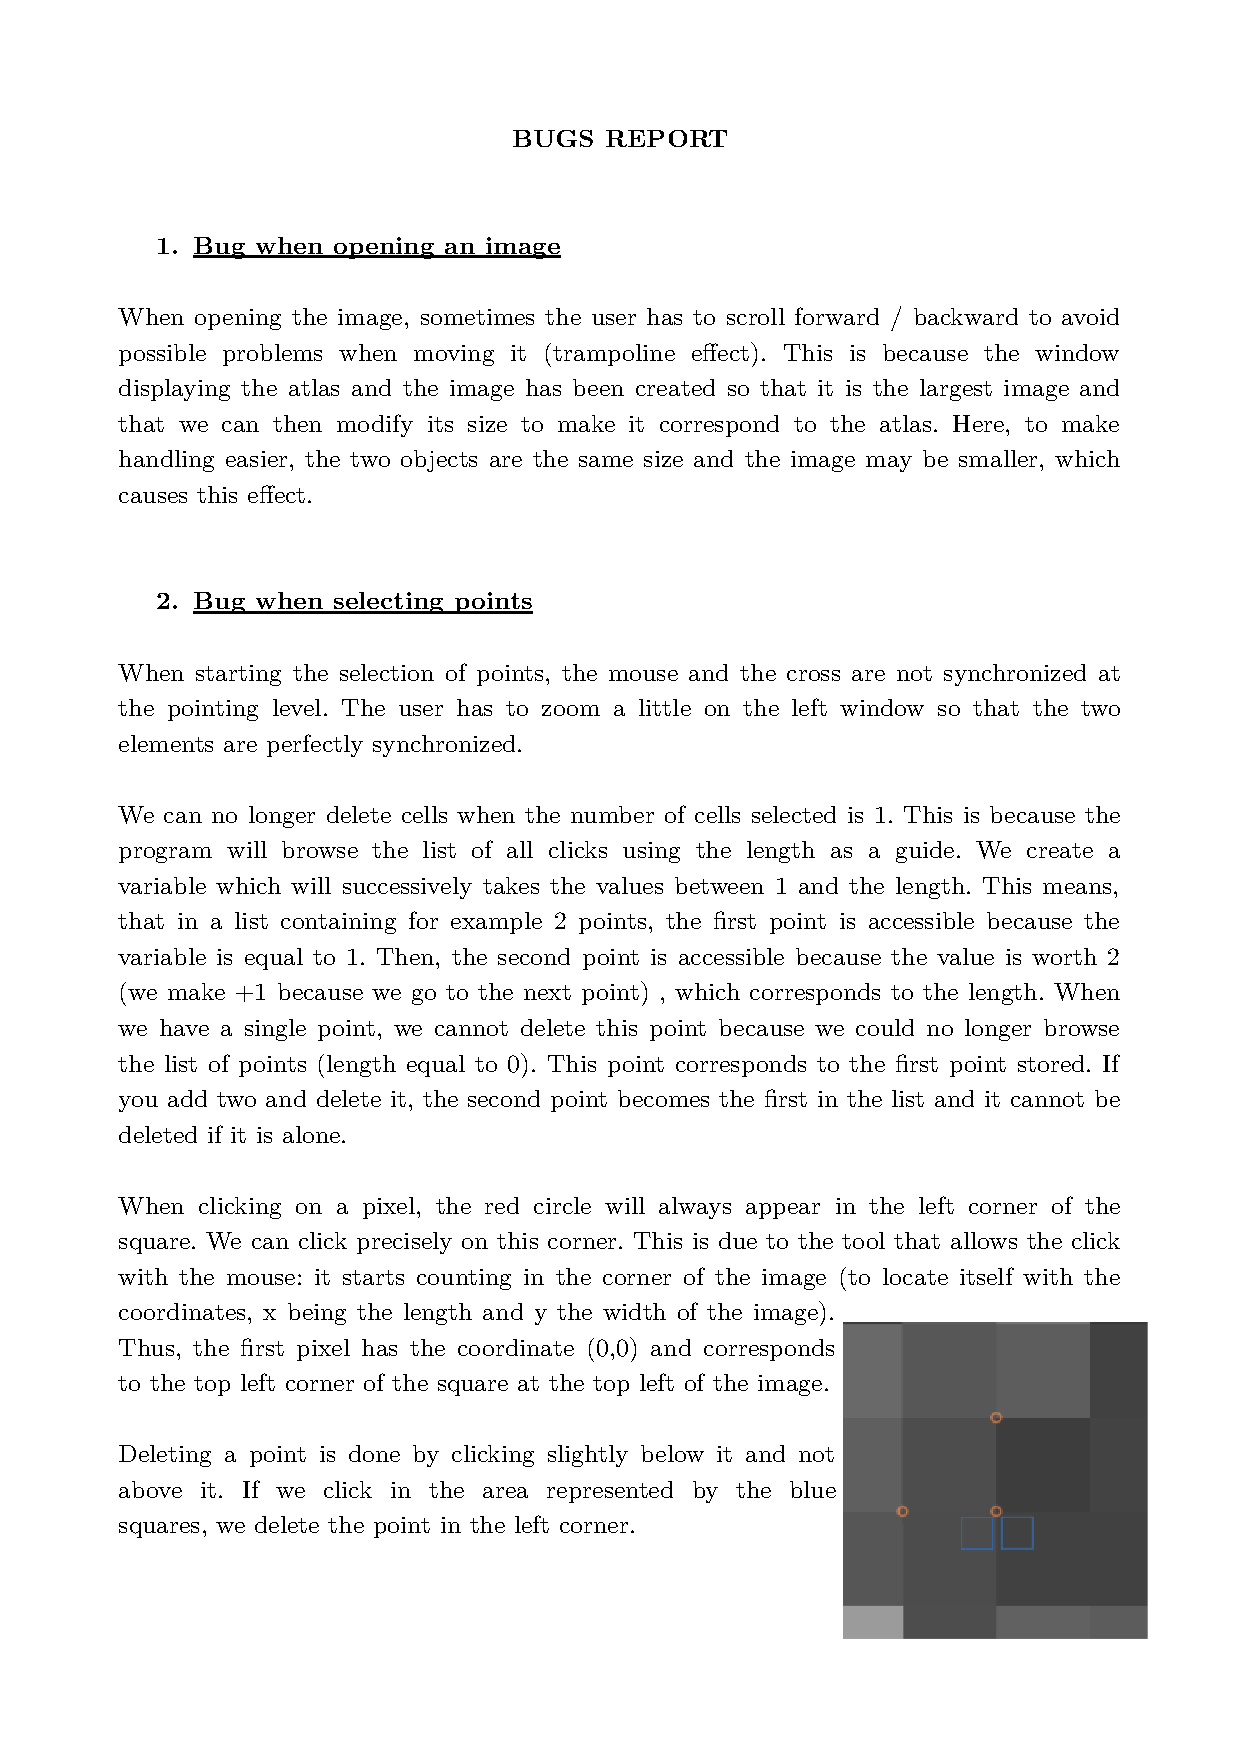
\includepdf[pages=1-2]{bugReport.pdf}

\end{document}

